\documentclass[hyperref={pdftex,pdfpagemode=none,pdfstartview=FitH},10pt,aspectratio=43]{beamer}
\usepackage[english]{babel}
\usepackage{times}
\usepackage{amsmath,amssymb}
\usepackage{subfigure,graphicx}
\usepackage{multirow,booktabs,diagbox,makecell}
\usepackage{tikz}
\usepackage{cases,booktabs}
\usetikzlibrary{arrows.meta}
\usetikzlibrary{shapes.arrows}
\usepackage{siunitx}
\usepackage{hyperref}
\usepackage{xcolor}

\newcommand{\SO}[1]{\ensuremath{\mathrm{SO}(#1)}}
\newcommand{\SE}[1]{\ensuremath{\mathrm{SE}(#1)}}
\newcommand{\so}[1]{\ensuremath{\mathfrak{so}(#1)}}
\newcommand{\Sph}{\ensuremath{\mathbb{S}}}
\newcommand{\norm}[1]{\ensuremath{\left\| #1 \right\|}}
\newcommand{\tr}[1]{\ensuremath{\mathrm{tr}\left( #1 \right)}}
\newcommand{\etr}[1]{\ensuremath{\mathrm{etr}\left( #1 \right)}}
\newcommand{\expect}[1]{\ensuremath{\mathrm{E}\left[ #1 \right]}}
\newcommand{\expectbar}[1]{\ensuremath{\bar{\mathrm{E}}\left[ #1 \right]}}
\newcommand{\cov}[2]{\ensuremath{\mathrm{cov}\left( #1, #2 \right)}}
\newcommand{\covbar}[2]{\ensuremath{\overline{\mathrm{cov}}\left( #1, #2 \right)}}
\newcommand{\expb}[1]{\ensuremath{\exp\left\{ #1 \right\}}}
\newcommand{\diff}{\ensuremath{\mathrm{d}}}
\newcommand{\diag}{\ensuremath{\mathrm{diag}}}

\makeatletter
\newcommand\approxsim{\mathchoice
	{\@approxsim {\displaystyle}      {1ex} }
	{\@approxsim {\textstyle}         {1ex} }
	{\@approxsim {\scriptstyle}       {.7ex}}
	{\@approxsim {\scriptscriptstyle} {.5ex}}}
\newcommand\@approxsim[2]{%
	\mathrel{%
		\ooalign{%
			$\m@th#1\sim$\cr
			\hidewidth$\m@th#1.$\hidewidth\cr
			\hidewidth\raise #2 \hbox{$\m@th#1.$}\hidewidth\cr
		}%
	}%
}
\makeatother

\setbeamerfont{footnote mark}{size=\tiny}

\definecolor{RoyalBlue}{rgb}{0.25,0.41,0.88}
\def\Emph{\textcolor{RoyalBlue}}

\definecolor{mygray}{gray}{0.9}
\definecolor{tmp}{rgb}{0.804,0.941,1.0}
%\setbeamercolor{numerical}{fg=black,bg=tmp}
\setbeamercolor{exact}{fg=black,bg=red}
\setbeamercolor{numerical}{fg=black,bg=mygray}

\mode<presentation> {
  \usetheme{Berkeley}
  \usefonttheme{serif}
  \setbeamercovered{transparent}
}

\setbeamertemplate{footline}%{split theme}
{%
  \leavevmode%
  \hbox{\begin{beamercolorbox}[wd=.5\paperwidth,ht=2.5ex,dp=1.125ex,leftskip=.3cm,rightskip=.3cm plus1fill]{author in head/foot}%
    \usebeamerfont{author in head/foot}\insertshorttitle
  \end{beamercolorbox}%
  \begin{beamercolorbox}[wd=.5\paperwidth,ht=2.5ex,dp=1.125ex,leftskip=.3cm plus1fill,rightskip=.3cm]{title in head/foot}%
    \usebeamerfont{title in
    head/foot}\insertframenumber/\inserttotalframenumber
  \end{beamercolorbox}}%
  \vskip0pt%
} \setbeamercolor{box}{fg=black,bg=yellow}

\title[]{Geometric Formulation of Uncertainties and Estimation \\ for Three-Dimensional Rotations}

\author[]{Weixin Wang \\ Advisor: Prof. Taeyoung Lee}

\institute[GWU]{\footnotesize\selectfont
Department of Mechanical and Aerospace Engineering\\
George Washington University, Washington DC\\$ $\\}

\date{\today}

\graphicspath{{./Figs/},{../figures/},{../figures/observability/}}

\newenvironment<>{varblock}[2][12cm]{
    \begin{center}
      \begin{minipage}{#1}
        \setlength{\textwidth}{#1}
          \begin{actionenv}#3
            \def\insertblocktitle{#2}
            \par
            \usebeamertemplate{block begin}}
  {\par
      \usebeamertemplate{block end}
    \end{actionenv}
  \end{minipage}
\end{center}}

\newenvironment<>{varblock2}[2][0.7\textwidth]{
          \begin{actionenv}#3
            \def\insertblocktitle{#2}
            \par
            \usebeamertemplate{block begin}}
  {\par
      \usebeamertemplate{block end}
    \end{actionenv}
}

\DeclareMathOperator*{\argmin}{arg\,min}
\DeclareMathOperator*{\argmax}{arg\,max}

%%%%%%%%%%%%%%%%%%%%%%%%%%%%%%%%%%%%%%%%%%%%%%%%%%%%%%%%%%%%

\begin{document}

\setcounter{framenumber}{-1}
\begin{frame}
	\titlepage
\end{frame}

\begin{frame}
	\frametitle{Overview}
	\tableofcontents
\end{frame}

\section{Motivation}

\begin{frame}
	\frametitle{Attitude Estimation in Engineering}
	
	\begin{itemize}
		\item 3D Rigid Body Attitude
		\begin{itemize}
			\item The orientation of a reference frame fixed to the rigid body.
			\item The space of 3D attitude: three dimensional special orthogonal group.
			
			\centerline{
				\begin{beamercolorbox}[wd=10cm,sep=0.0cm,center,rounded=true,shadow=true]{numerical}
					\small
					\vspace{-0.3cm}
					\begin{equation*}
						\SO{3} = \{R\in\mathbb{R}^{3\times 3} \,|\, RR^T = I_{3\times 3},\, \det(R) = 1\}.
					\end{equation*}
					\vspace{-0.5cm}
				\end{beamercolorbox}
			}
			
			\item Rotation matrix $R\in\SO{3}$: transform the coordinates of a vector from the \Emph{body-fixed frame} $x^B$ to \Emph{inertial frame} $x^I$.
			
			\centerline{
				\begin{beamercolorbox}[wd=10cm,sep=0.0cm,center,rounded=true,shadow=true]{numerical}
					\small
					\vspace{-0.3cm}
					\begin{equation*}
						x^I = Rx^B
					\end{equation*}
					\vspace{-0.5cm}
				\end{beamercolorbox}
			}
		\end{itemize}
	
		\vspace{0.3cm}
		\item Applications in Engineering
		\begin{itemize}
			\item Alignment of two satellites: laser communication.
			\item Attitude control for UAVs.
			\item Inertial navigation.
		\end{itemize}
	\end{itemize}
\end{frame}

\begin{frame}
	\frametitle{Uncertainty for 3D Attitude}
	
	\begin{itemize}
		\item State Estimation of a Dynamical System
		\begin{itemize}
			\item Uncertainty Propagation: propagete the mean and covariance matrix of the state through the kinematic equations.
			\item Measurement Update: use new measurements to correct propagation errors.
			\item Covariance matrices are used to weigh the propagation and measurement noises.
		\end{itemize}
	
		\vspace{0.3cm}
		\item What is Covariance Matrix for 3D Rotation?
		\begin{itemize}
			\item Covariance for lower dimensional parameterizations:
			\begin{itemize}
				\item Three dimensional: Euler angles, (modified) Rodrigues parameters, etc.
				\item Four dimensional: Unit quaternions.
			\end{itemize}
		
			\item Problems with three dimensional parameterizations:
			\begin{itemize}
				\item \Emph{Singularities}: such as gimbal lock for Euler angles.
				\item The Lebesgue measure on $\mathbb{R}^3$ is no longer uniform when transformed to $\SO{3}$.
			\end{itemize}
		
			\item Problems with quaternions:
			\begin{itemize}
				\item The \Emph{unit norm constraint} makes the covariance matrix singular.
			\end{itemize}
		\end{itemize}
	\end{itemize}
\end{frame}

\begin{frame}
	\frametitle{Multiplicative Extended Kalman Filter}
	\begin{itemize}
		\item Covariance Matrix for \Emph{Attitude Error}
		
		\centerline{
			\begin{beamercolorbox}[wd=10cm,sep=0.0cm,center,rounded=true,shadow=true]{numerical}
				\small
				\vspace{-0.3cm}
				\begin{equation*}
					q_t = q \otimes q\{\delta v\}.
				\end{equation*}
				\vspace{-0.5cm}
			\end{beamercolorbox}
		}
		
		\begin{itemize}
			\item $q_t,q\in\Sph^3$: true and estimated attitude represented by unit quaternions.
			\item $q\{\delta v\} \in \Sph^3$: error attitude expressed as a rotation vector $\delta v\in\mathbb{R}^3$.
			\item $\delta v \sim \mathcal{N}(0,\Sigma)$, where $\Sigma\in\mathbb{R}^{3\times 3}$ is the covariance matrix, representing the uncertainty of the attitude.
			\begin{itemize}
				\item $\delta v$ is three dimensional.
				\item $\delta v$ is usually small, so singularity is avoided.
			\end{itemize}
		\end{itemize}
	
		\vspace{0.3cm}
		\item Multiplicative Extended Kalman Filter
		\begin{itemize}
			\item Using Gaussian distribution to model the uncertainty of attitude error.
			\item Problems: \Emph{not suitable for large uncertainty}
			\begin{itemize}
				\item Linearization error.
				\item Wrapping error.
			\end{itemize}
		\end{itemize}
	\end{itemize}
\end{frame}

\begin{frame}
	\frametitle{Wrapping Errors for Gaussian Distribution}
	
	\begin{itemize}
		\item Attitude Error is in the \Emph{Tangent Space} of $\SO{3}$.
		
		\vspace{0.4cm}
		\item Problems: not suitable for large uncertainty
		\begin{itemize}
			\item Inherent \Emph{non-linearity}: $\SO{3}$ is a curved manifold.
			\item \Emph{Wrapping errors} for cyclic tangent space.
		\end{itemize}
		
		\vspace{-0.1cm}
	
		\centerline{
			\begin{tikzpicture}
				\node[opacity=1.0,outer sep=0pt,inner sep=0pt] at (0,0) {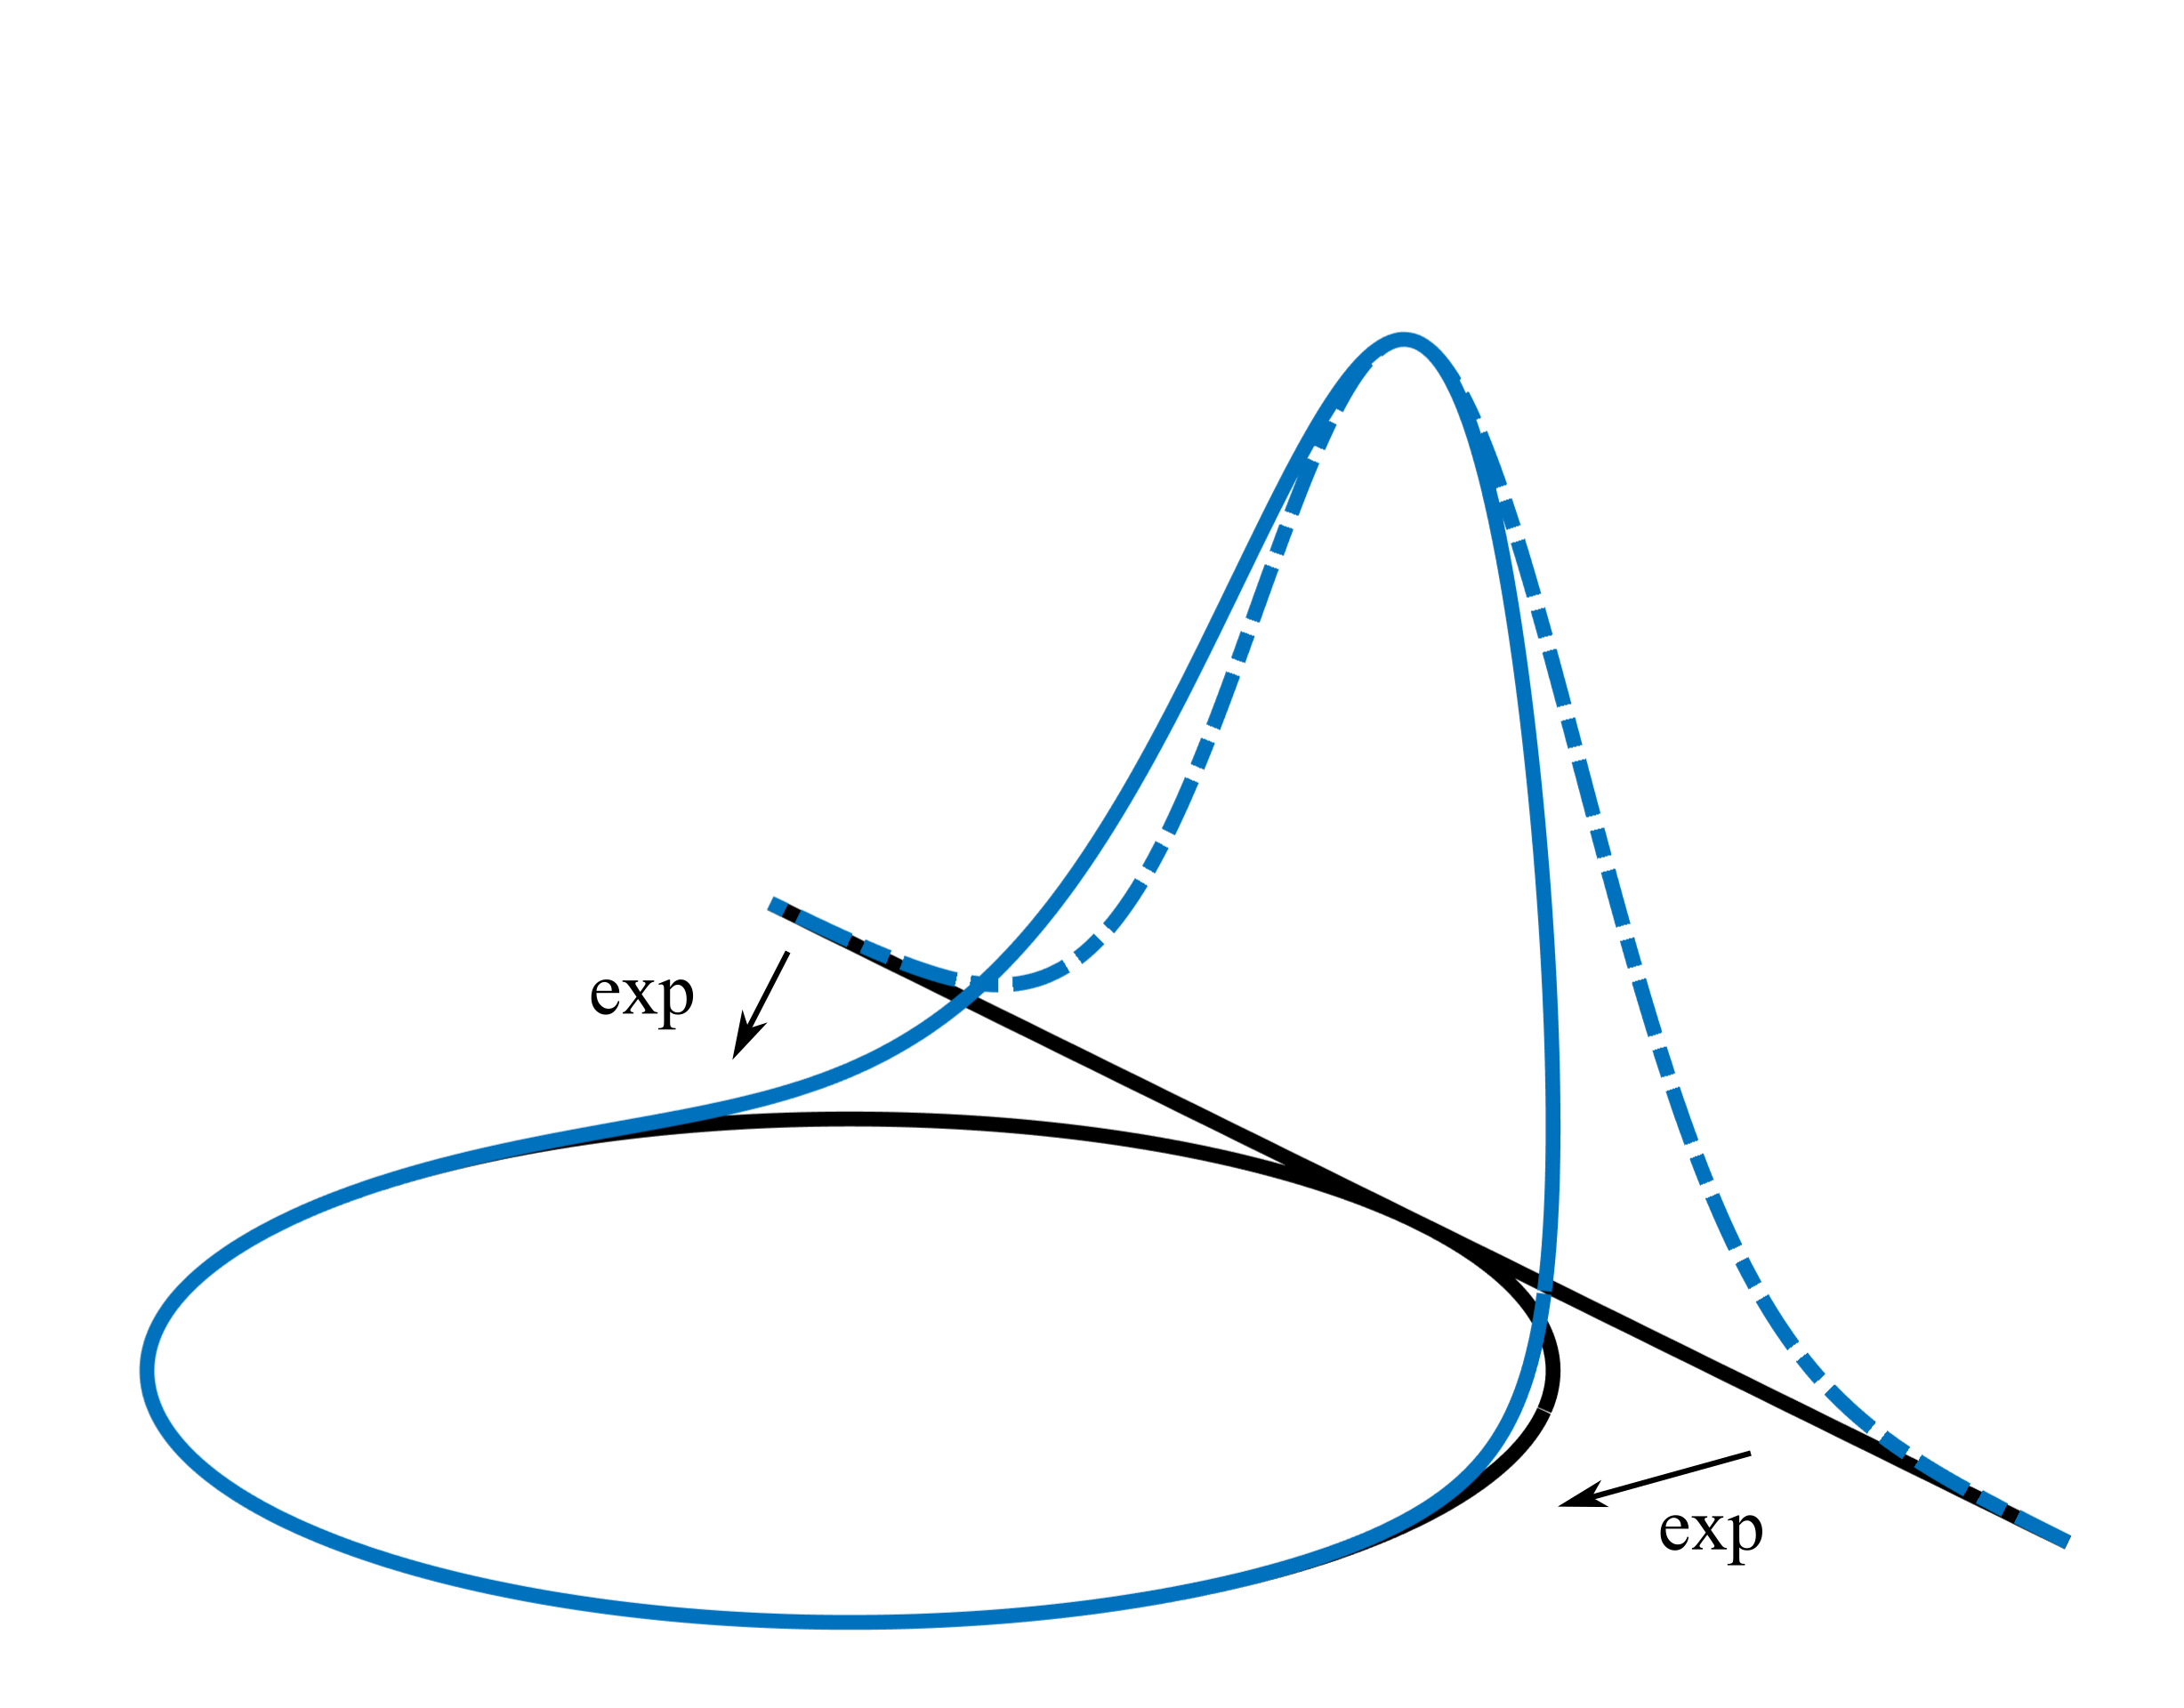
\includegraphics[scale=0.4]{circle_density_edited}};
				\node[opacity=1.0,outer sep=0pt,inner sep=0pt] at (5.2,-0.2) {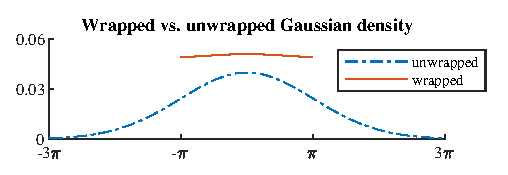
\includegraphics[scale=0.7]{wrapping}};
			\end{tikzpicture}
		}
	
		\pause
		\item A probability distribution \Emph{directly defined on $\SO{3}$} could avoid these issues.
	\end{itemize}
\end{frame}

\section{Matrix Fisher Distribution}

\begin{frame}
	\frametitle{Matrix Fisher Distribuiton}
	
	\begin{itemize}
		\item Matrix Fisher Distribution: Defined on $\SO{3}$
		\begin{itemize}
			\item Construction: condition a Gaussian distribution from $\mathbb{R}^9$ to $\SO{3}$.
			\item Density function for $R\sim\mathcal{M}(F)$:
			
			\centerline{
				\begin{beamercolorbox}[wd=10cm,sep=0.0cm,center,rounded=true,shadow=true]{numerical}
					\small
					\vspace{-0.3cm}
					\begin{equation*}
						p(R) = \frac{1}{c(F)} \expb{\tr{FR^T}}.
					\end{equation*}
					\vspace{-0.4cm}
				\end{beamercolorbox}
			}
		
			\begin{itemize}
				\item $F\in\mathbb{R}^{3\times 3}$ is the parameter, $c(F)\in\mathbb{R}$ is the normalizing constant.
			\end{itemize}
		\end{itemize}
	
		\vspace{0.2cm}
		\item Bingham Distribution: Defined on $\Sph^3$
		\begin{itemize}
			\item \Emph{Equivalent to the matrix Fisher distribution} under the homomorphism from $\SO{3}$ to $\Sph^3$.
		\end{itemize}
	\end{itemize}
	
	\vspace{0.2cm}
	\only<1>{\centerline{
			\begin{tikzpicture}
				\node[opacity=1,outer sep=0pt,inner sep=0pt] at (0,0) {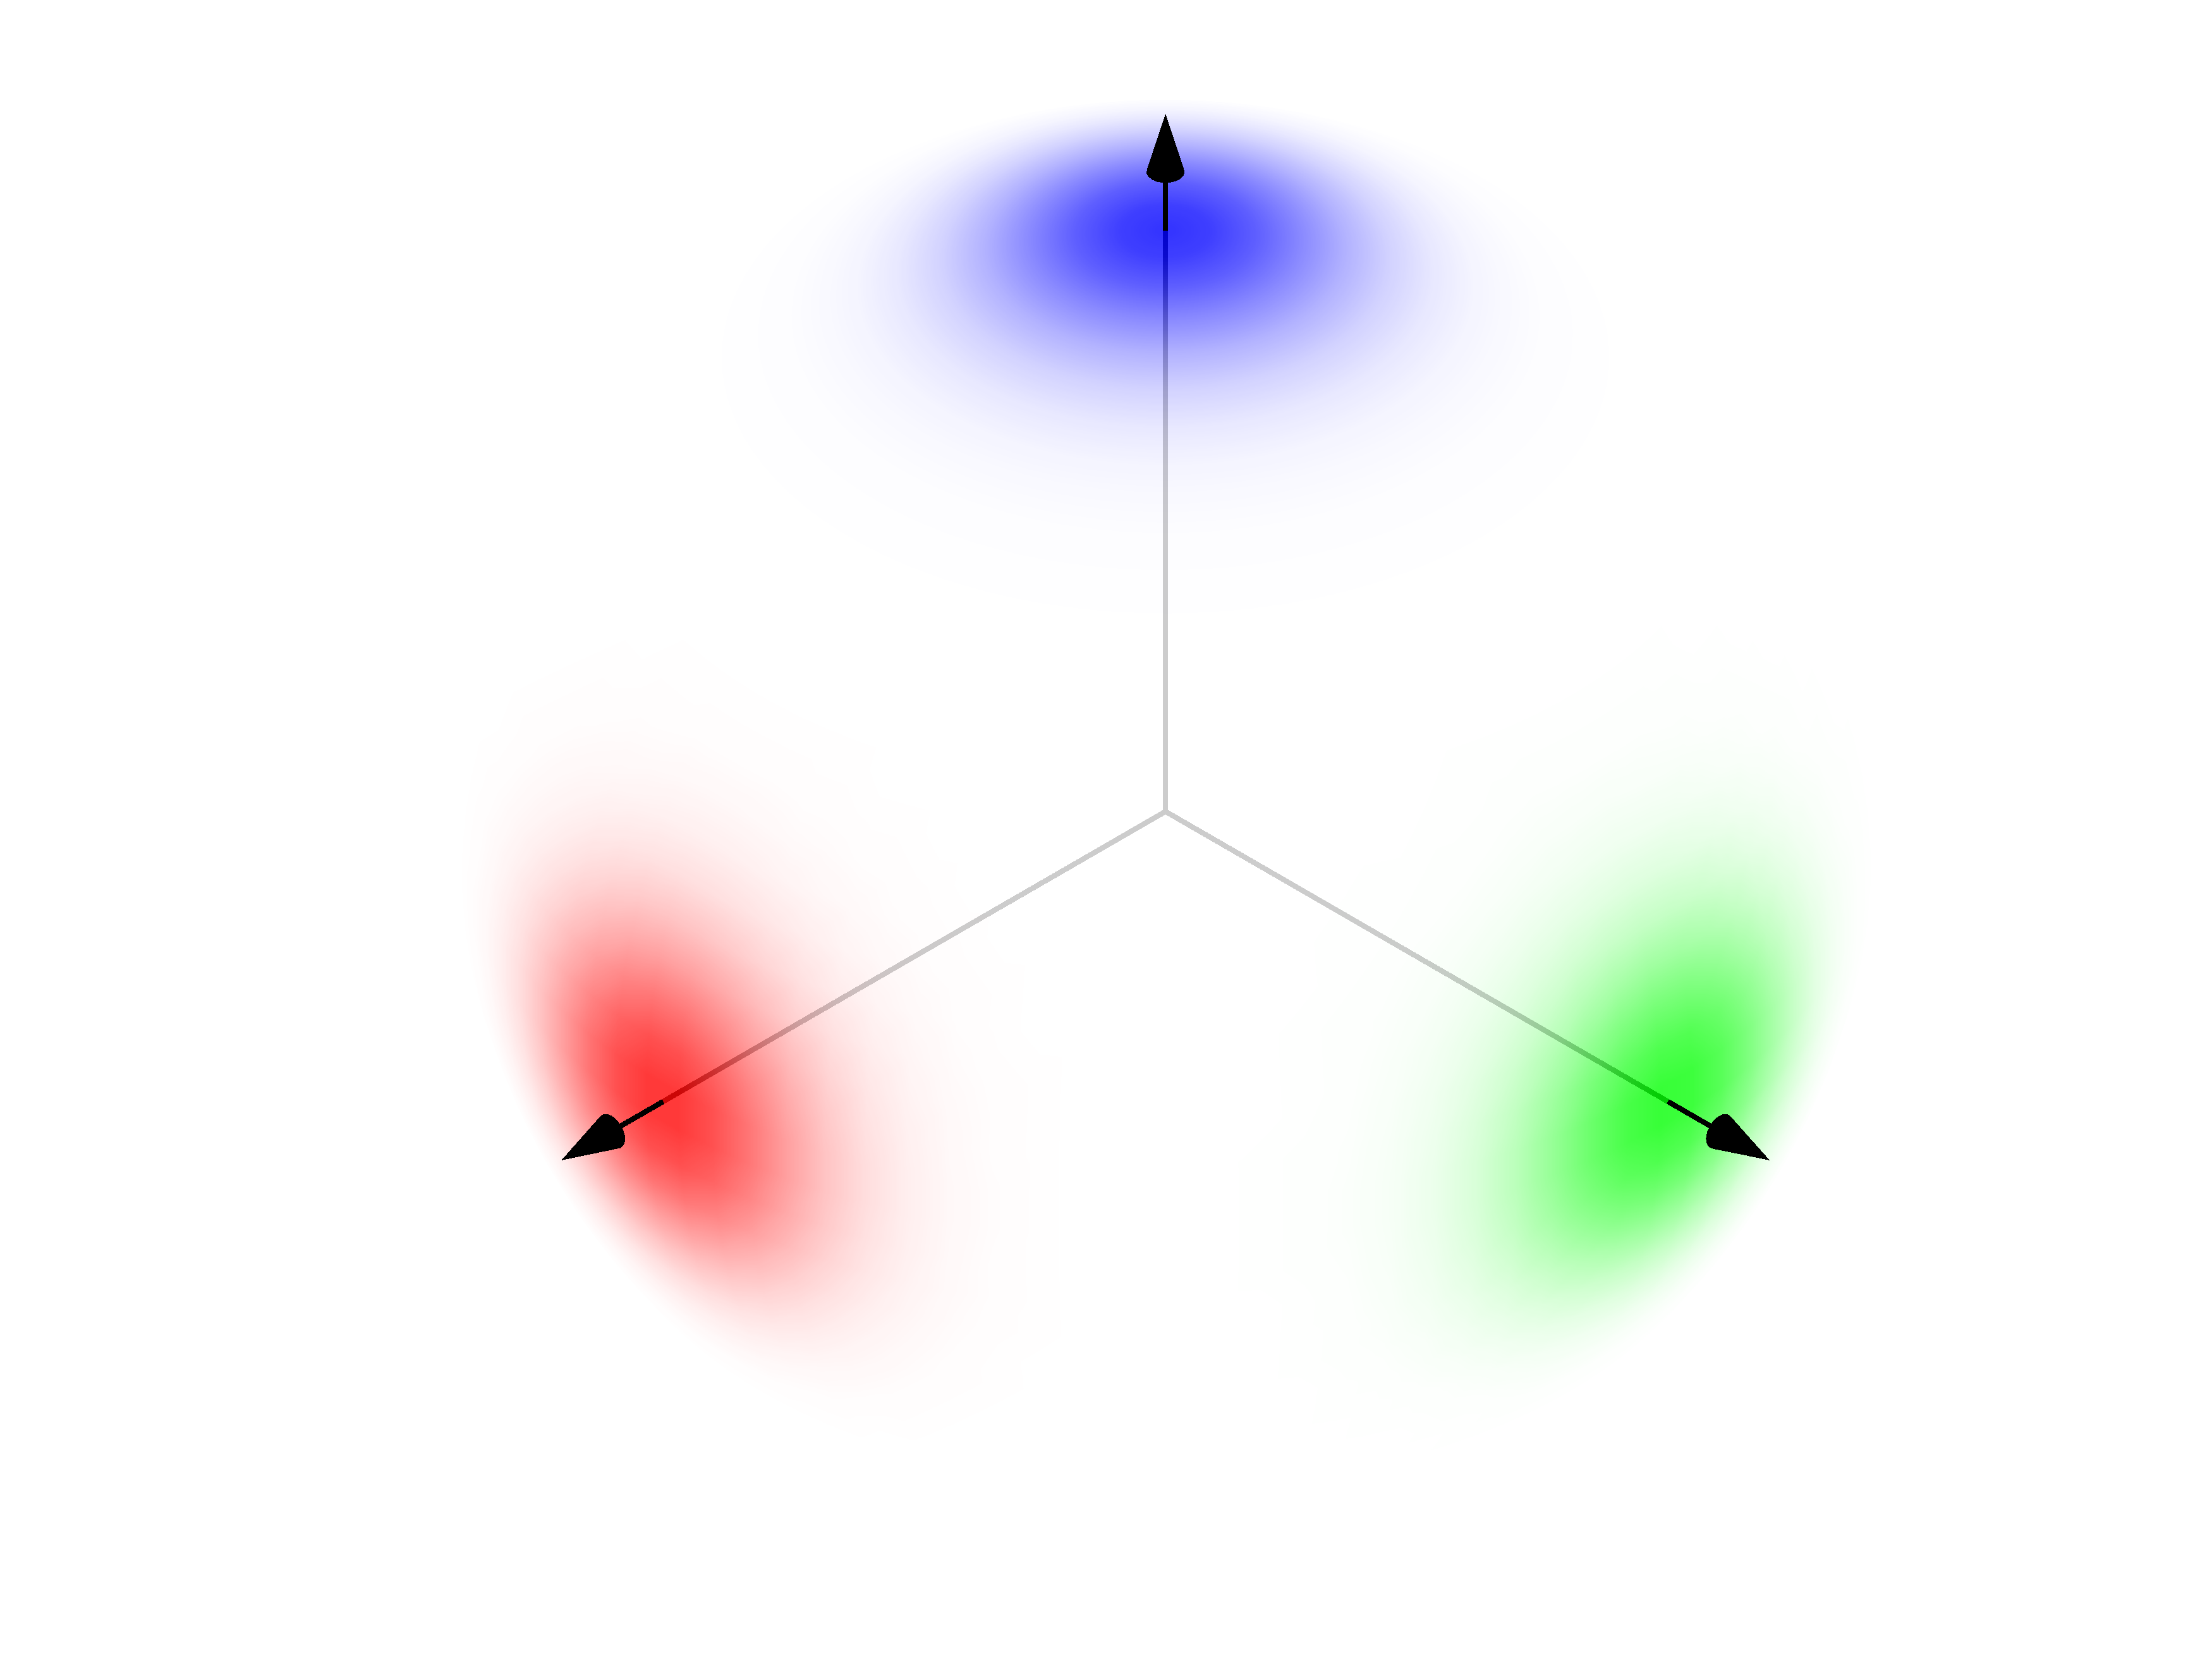
\includegraphics[scale=0.2]{MFDensity1}};
				\node[opacity=1,outer sep=0pt,inner sep=0pt] at (3,0) {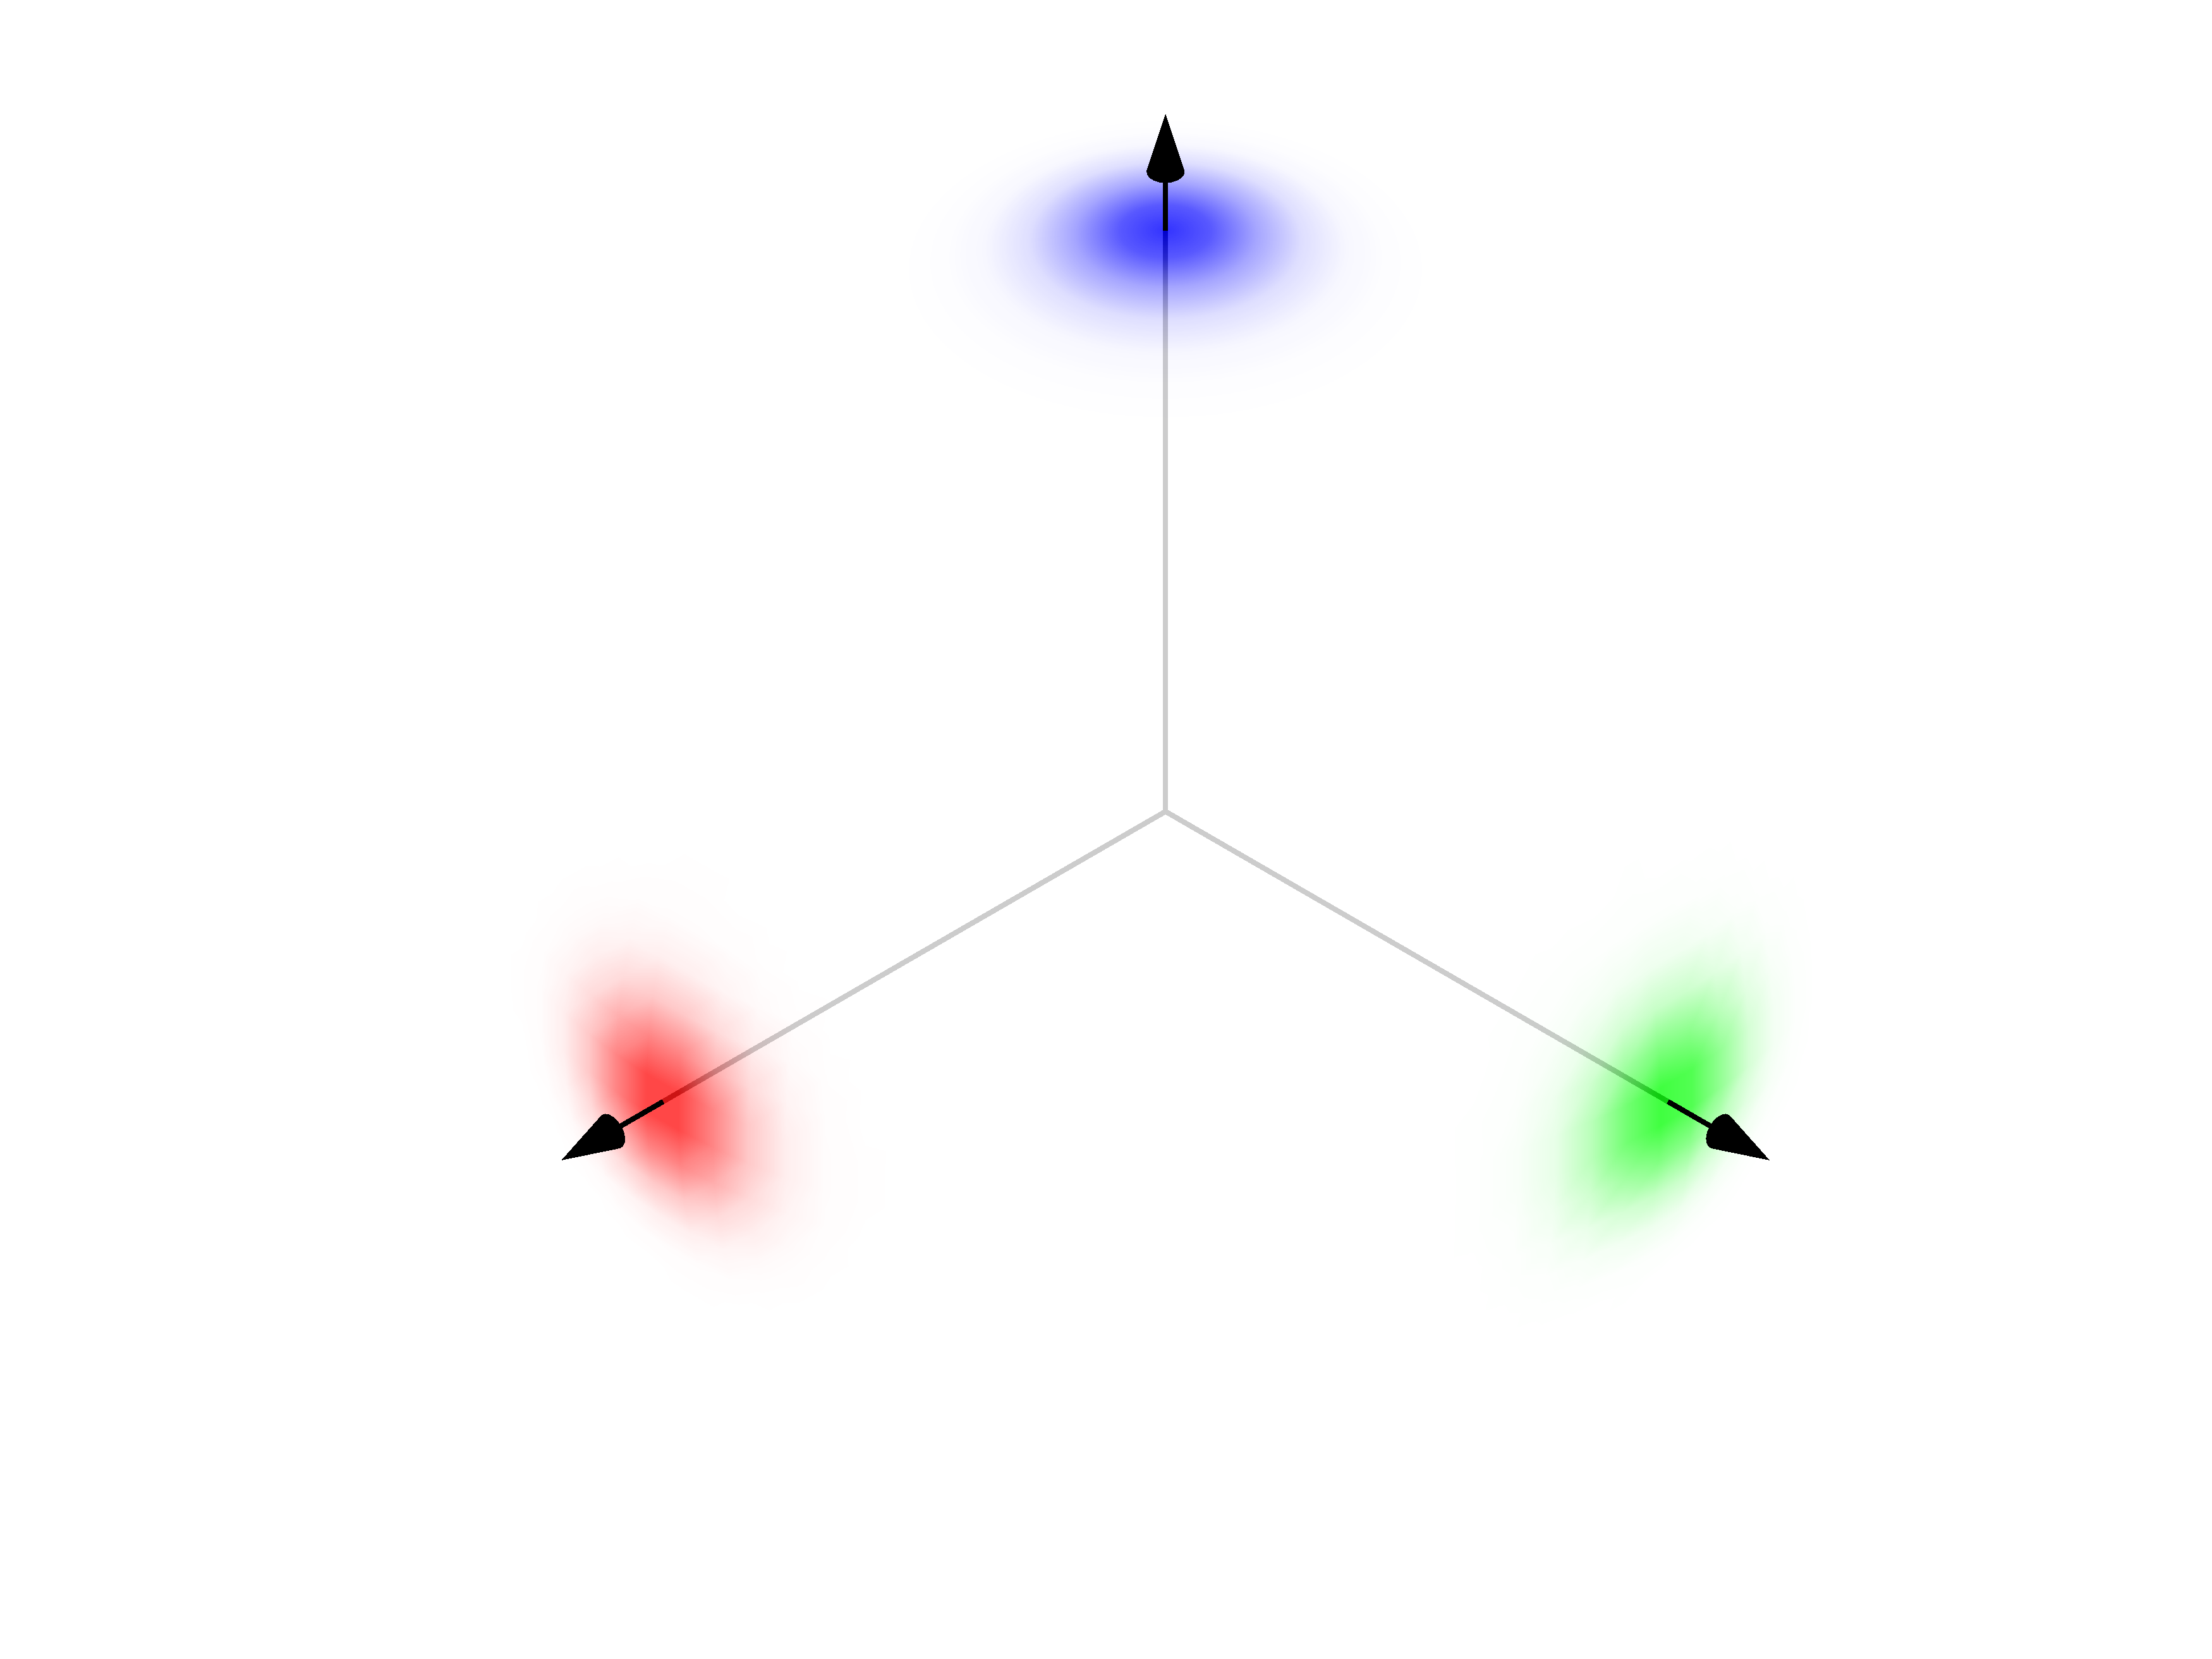
\includegraphics[scale=0.2]{MFDensity2}};
				\node[opacity=1,outer sep=0pt,inner sep=0pt] at (6,0) {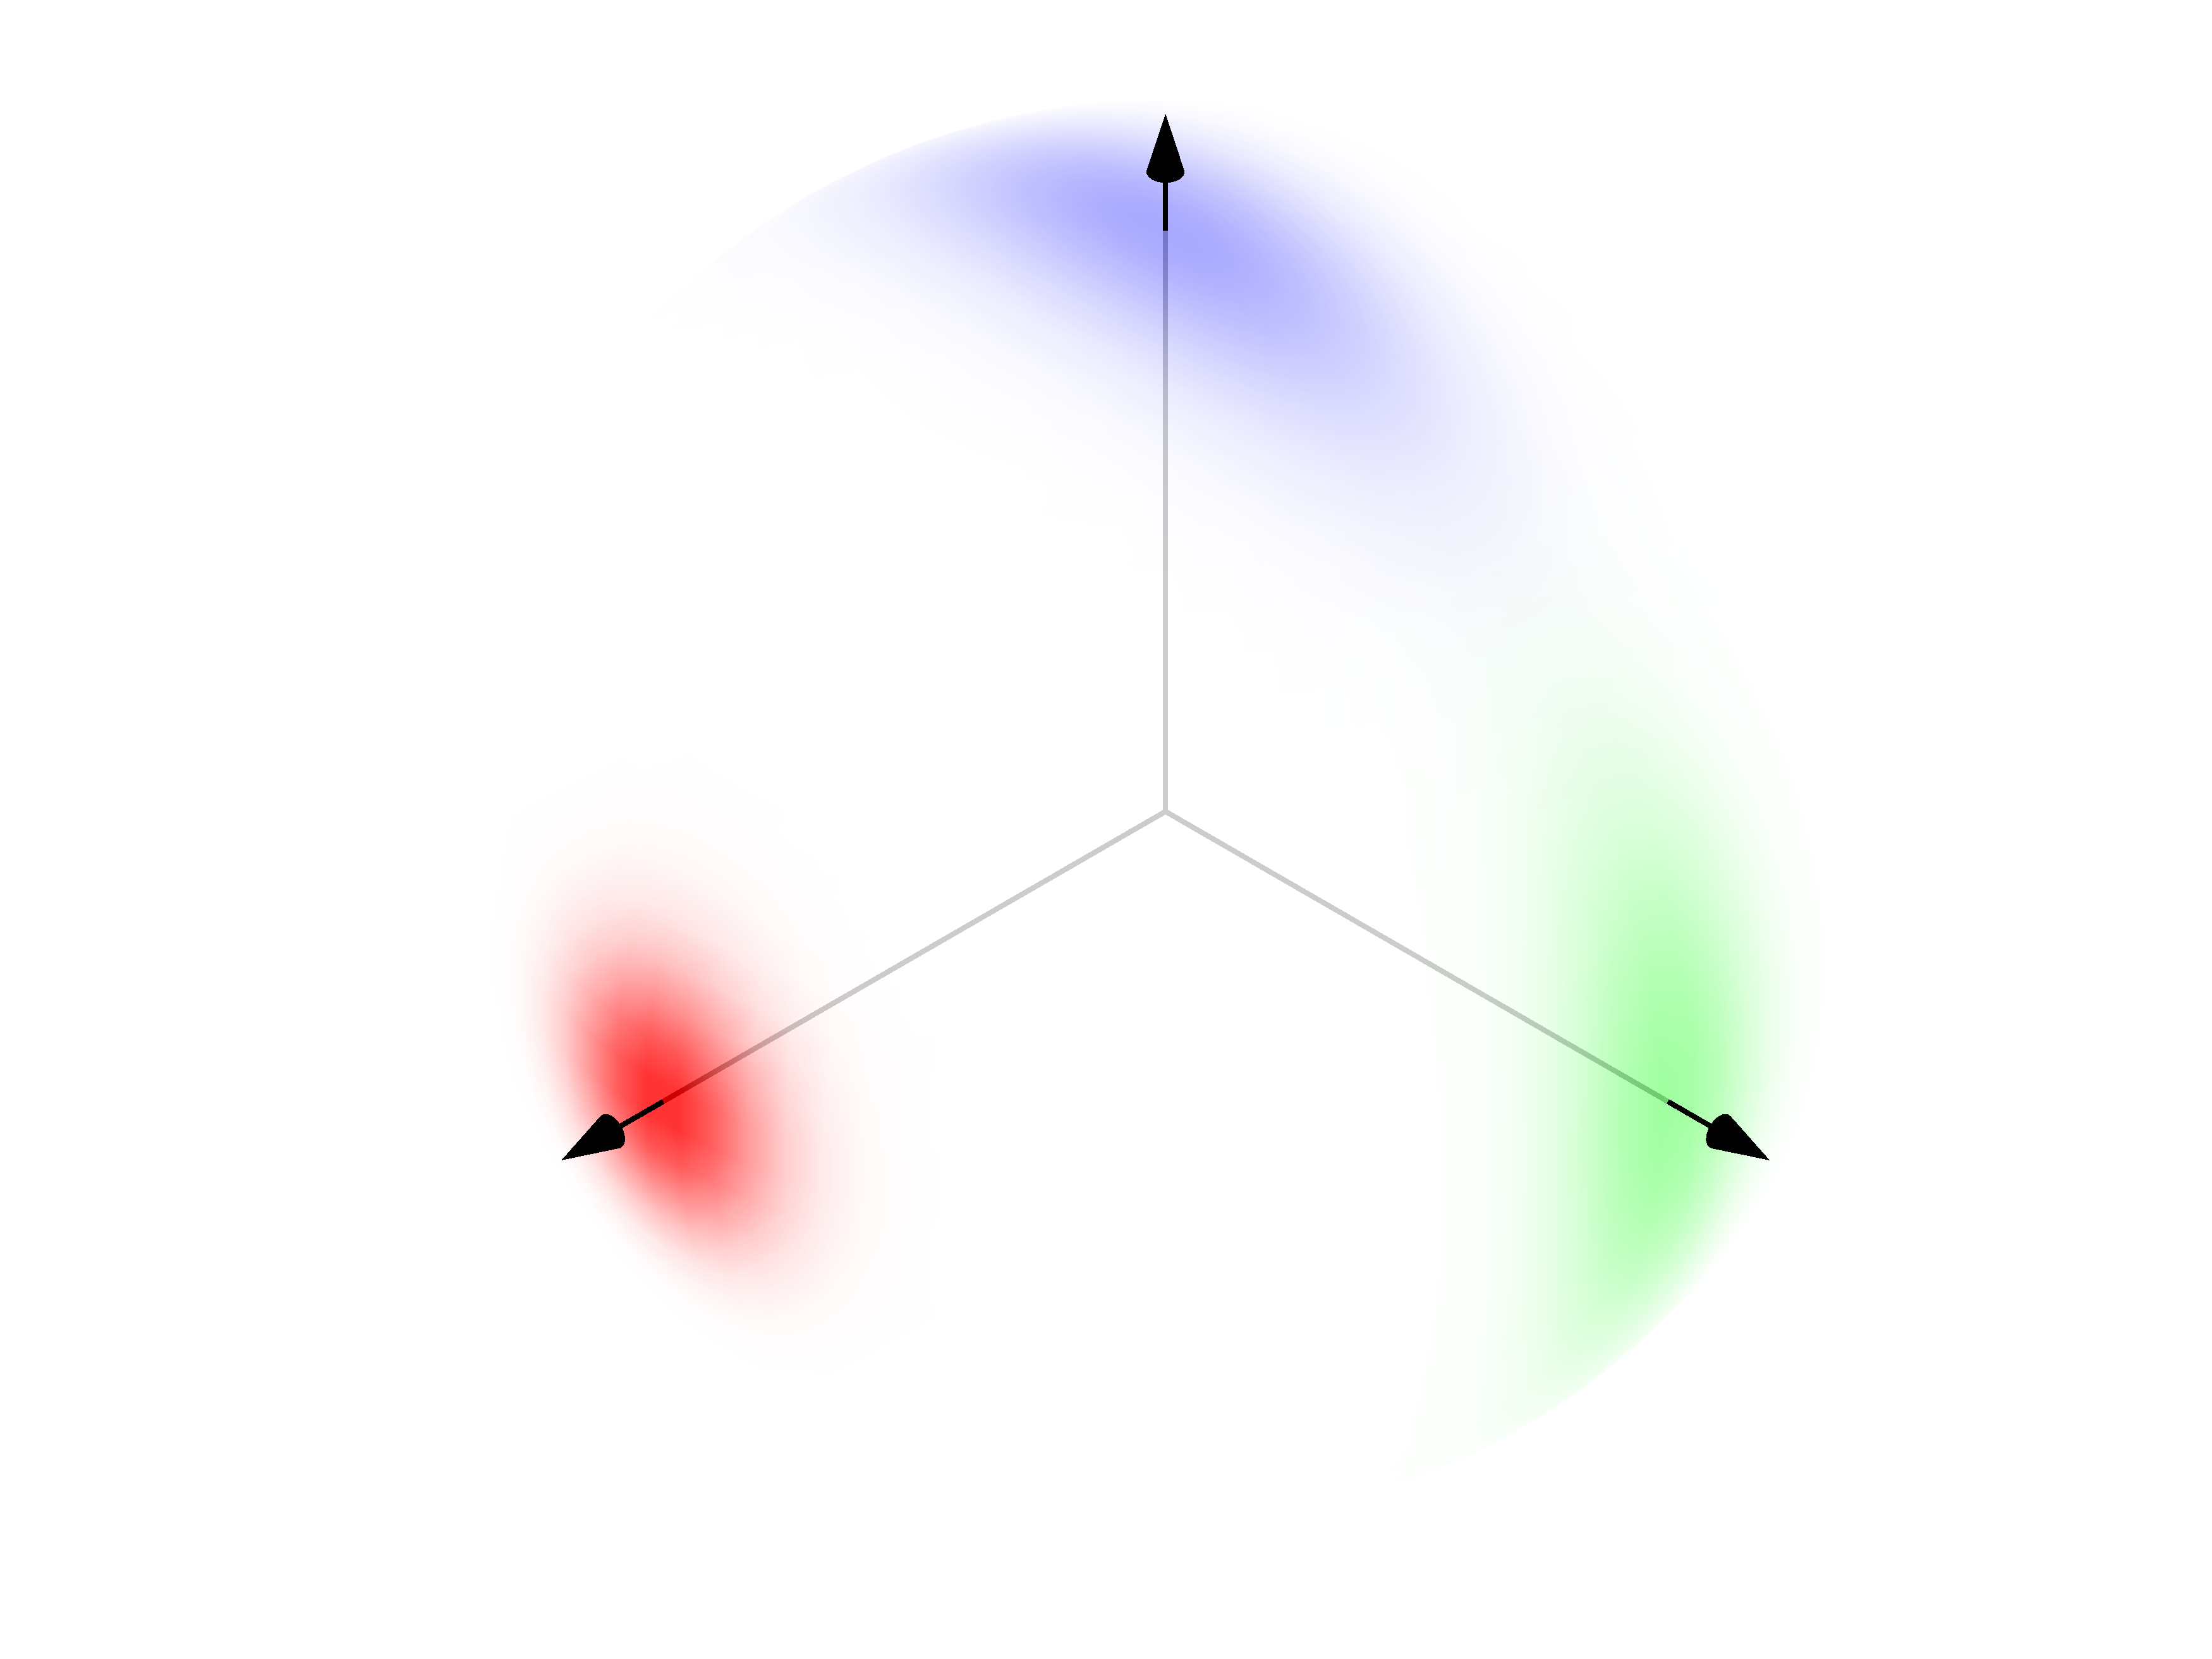
\includegraphics[scale=0.2]{MFDensity3}};
			\end{tikzpicture}
	}}
\end{frame}

\begin{frame}
	\frametitle{Properties}
	
	\begin{itemize}
		\item Shape of the Density Function
		\begin{itemize}
			\item proper singular value decomposition (pSVD) of the parameter: $F = USV^T$.
			\item \Emph{Mean attitude}: $M = UV^T$ (uni-modal).
			\item \Emph{Principal axes}:
			\begin{itemize}
				\item Columns of $U$ in the inertial frame.
				\item Columns of $V$ in the body-fixed frame of the mean attitude $M$.
			\end{itemize}
			\item \Emph{Dispersion}: $s_i+s_j$ specifies the dispersion along the $k$-th principal axis, for $i\neq j\neq k$.
			\item Analogous to a Gaussian distribution.
		\end{itemize}
	
		\vspace{0.2cm}
		\item Maximum Likelihood Estimation (MLE) for Parameters
		\begin{itemize}
			\item Moments
			
			\centerline{
				\begin{beamercolorbox}[wd=10cm,sep=0.0cm,center,rounded=true,shadow=true]{numerical}
					\small
					\vspace{-0.3cm}
					\begin{equation*}
						\expect{R} = UDV^T, \qquad \qquad d_i = \frac{1}{c(S)} \frac{\partial c(S)}{\partial s_i}.
					\end{equation*}
					\vspace{-0.4cm}
				\end{beamercolorbox}
			}
		
			\item MLE for $U,V\in\SO{3}$: the pSVD of $\expect{R} = USV^T$.
			\item MLE for $S$: solving $d_i = \frac{1}{c(S)} \frac{\partial c(S)}{\partial s_i}$ from $D$.
		\end{itemize}
	\end{itemize}
\end{frame}

\begin{frame}
	\frametitle{Central Moments}
	\begin{itemize}
		\item Motivation
		\begin{itemize}
			\item Designing Bayesian filters using matrix Fisher distribution sometimes needs to evaluate its higher order moments.
		\end{itemize}

		\vspace{0.2cm}
		\item Central Moments for Matrix Fisher Distribution: $Q = U^TRV$
		
		\centerline{
			\begin{beamercolorbox}[wd=10cm,sep=0.0cm,center,rounded=true,shadow=true]{numerical}
				\small
				\vspace{-0.3cm}
				\begin{equation*}
					\expect{Q_{i_1j_1}\cdots Q_{i_nj_n}} = \frac{1}{c(S)} \left. \frac{\partial c(S+T)}{\partial T_{i_1j_1} \cdots \partial T_{i_nj_n}} \right|_{T = 0}.
				\end{equation*}
				\vspace{-0.4cm}
			\end{beamercolorbox}
		}
	
		\begin{itemize}
			\item $\expect{Q_{i_1j_1}\cdots Q_{i_nj_n}} = 0$ if $\{i_k,j_k\}_{k=1}^n$ has odd number of 1, 2, or 3.
			\item $\expect{Q_{i_1j_1}\cdots Q_{i_nj_n}} = \expect{Q_{j_1i_1} \cdots Q_{j_ni_n}}$.
		\end{itemize}
	
		\vspace{0.2cm}
		\item Computation
		\begin{itemize}
			\item $\expect{Q_{i_1j_1}\cdots Q_{i_nj_n}}$ is a linear combination of the derivatives of $c(S)$ up to $n$-th order.
			\item The coefficients and derivatives of $c(S)$ can be calculated recursively.
			\item The recursion starts from $c(S)$ and its first order derivatives $\frac{\partial c(S)}{\partial s_i}$.
		\end{itemize}
	\end{itemize}
\end{frame}

\begin{frame}
	\frametitle{Highly Concentrated Approximations}
	
	\begin{itemize}
		\item Motivation
		\begin{itemize}
			\item Evaluating the normalizing constant $c(S)$ and its derivatives is hard.
			\item The MLE $d_i = \frac{1}{c(S)} \frac{\partial c(S)}{\partial s_i}$ is very hard to solve.
		\end{itemize}
	
		\vspace{0.2cm}
		\only<1>{
			\item Highly Concentrated in Three Degrees of Freedom
			\begin{theorem}
				Let $R\sim\mathcal{M}(F)$, where $F=USV^T$ is the pSVD of $F$.
				Suppose $s_2+s_3\gg 0$.
				Let $Q = U^TRV = \exp\left(\hat{\eta}\right)$, then \Emph{$\eta \approxsim \mathcal{N}\big( 0,\allowbreak (\tr{S}I_{3\times 3}-S)^{-1} \big)$}.
			\end{theorem}
		
			\begin{itemize}
				\item The matrix Fisher distribution is approximated by a Gaussian distribution in $\mathbb{R}^3$.
			\end{itemize}
		}
	
		\only<2>{
			\item Highly Concentrated in Three Degrees of Freedom
			
			\begin{itemize}
				\item Approximations of $c(S)$ and its derivatives ($i\neq j\neq k$):
				
				\centerline{
					\begin{beamercolorbox}[wd=10cm,sep=0.0cm,center,rounded=true,shadow=true]{numerical}
						\small
						\vspace{-0.3cm}
						\begin{align*}
							c(S) &\approx \frac{\etr{S}}{\sqrt{8\pi(s_1+s_2)(s_1+s_3)(s_2+s_3)}} \label{eqn:MF-normalizing-approx1} \\
							\frac{1}{c(S)} \frac{\partial c(S)}{\partial s_i} &\approx 1 - \frac{1}{2}\left( \frac{1}{s_i+s_j} + \frac{1}{s_i+s_k} \right), \label{eqn:MF-S2D-approx1}
						\end{align*}
						\vspace{-0.4cm}
					\end{beamercolorbox}
				}
			\end{itemize}
		}
	
		\only<3>{
			\item Highly Concentrated in Two Degrees of Freedom
			\begin{theorem}
				Let $R\sim\mathcal{M}(F)$, where $F=USV^T$ is the pSVD of $F$.
				Suppose $s_1+s_3\gg s_2+s_3 \geq 0$.
				Let $Q = U^TRV = \exp\left(\hat{\eta}\right) \exp\left(\hat{\eta}'\right)$, where $\eta = [0, \eta_2, \eta_3]^T$, and $\eta' = [\eta_1, 0, 0]^T$.
				Then \Emph{$\eta_3 \approxsim \mathcal{VM}(0,s_2+s_3)$}, and \Emph{$[\eta_2, \eta_3]^T  \approxsim \mathcal{N}\left( 0, \diag\left( \tfrac{1}{s_1+s_3}, \tfrac{1}{s_1+s_2} \right) \right)$}, and they are approximately independent.
			\end{theorem}
		
			\begin{itemize}
				\item The matrix Fisher distribution is approximated by a combination of Gaussian distribution in $\mathbb{R}^2$, and a von Mises distribution on $\Sph^1$.
			\end{itemize}
		}
	
		\only<4>{
			\item Highly Concentrated in Two Degrees of Freedom
			\begin{itemize}
				\item Approximations of $c(S)$ and its derivatives ($j\in\{2,3\}$):
				
				\centerline{
					\begin{beamercolorbox}[wd=10cm,sep=0.0cm,center,rounded=true,shadow=true]{numerical}
						\small
						\vspace{-0.3cm}
						\begin{align*}
							c(S) &\approx \frac{\exp(s_1)I_0(s_2+s_3)}{2\sqrt{(s_1+s_2)(s_1+s_3)}}, \label{eqn:MF-normalizing-approx2} \\
							\frac{1}{c(S)}\frac{\partial c(S)}{\partial s_1} &\approx 1 - \frac{1}{2}\left( \frac{1}{s_1+s_2} + \frac{1}{s_1+s_3} \right), \label{eqn:MF-S2D-approx2-1} \\
							\frac{1}{c(S)}\frac{\partial c(S)}{\partial s_j} &\approx \frac{I_1(s_2+s_3)}{I_0(s_2+s_3)} - \frac{1}{2}\frac{1}{s_1+s_j}, \label{eqn:MF-S2D-approx2-2}
						\end{align*}
						\vspace{-0.4cm}
					\end{beamercolorbox}
				}
			\end{itemize}
		}
	\end{itemize}
\end{frame}

\section{Matrix Fisher--Gaussian Distribution}

\begin{frame}
	\frametitle{Correlation Between $\SO{3}$ and $\mathbb{R}^n$}
	
	\begin{itemize}
		\item Examples
		\begin{itemize}
			\item Attitude estimation: correlation between attitude and gyroscope bias.
			\item Inertial navigation: correlation between attitude and position.
			\item SLAM: correlation between attitude and landmark locations.
		\end{itemize}
	
		\item Existing Models
		\begin{itemize}
			\item In Markley 2006\footnote{\tiny F.~L. Markley, ``Attitude filtering on $\mathrm{SO}(3)$,'' \emph{The Journal of the Astronautical Sciences}, vol.~54, no. 3-4, pp. 391--413, 2006.}, the matrix Fisher distribution on $\SO{3}$ is combined with Gaussian distribution in $\mathbb{R}^n$.
			
			\item In Darling 2016\footnote{\tiny J.~E. Darling and K.~J. DeMars, ``Uncertainty propagation of correlated quaternion and {E}uclidean states using the {G}auss-{B}ingham density,'' \emph{Journal of Advances in Information Fusion}, vol.~11, no.~2, pp. 1--20, 2016}, the Bingham distribution on $\Sph^3$ is combined with Gaussian distribution in $\mathbb{R}^n$.
			
			\item Problems:
			\begin{itemize}
				\item These models do not have a generic geometric construction.
				\item Their MLEs are complicated and need numerical optimizations, so they are \Emph{not suitable for real time implementations}.
			\end{itemize}
		\end{itemize}
	\end{itemize}
\end{frame}

\begin{frame}
	\frametitle{Matrix Fisher--Gaussian Distribution}
	
	\begin{itemize}
		\item Matrix Fisher--Gaussian Distribution (MFG)
		\begin{itemize}
			\item Density: $\SO{3}\times\mathbb{R}^n \ni (R,x) \sim \mathcal{MG}(\mu,\Sigma,P,U,S,V)$ if
			
			\centerline{ \hspace{-0.2cm}
				\begin{beamercolorbox}[wd=10cm,sep=0.0cm,center,rounded=true,shadow=true]{numerical}
					\small
					\vspace{-0.4cm}
					\begin{equation*}
						f(R,x) = \tfrac{1}{c(S)\sqrt{(2\pi)^n\mathrm{det}({\Sigma}_c)}} \exp\left\{-\frac{1}{2}(x-\mu_c)^T\Sigma_c^{-1}(x-\mu_c)\right\} \exp\left\{\tr{FR^T}\right\}
					\end{equation*}
					\vspace{-0.4cm}
				\end{beamercolorbox}
			}
		
			\begin{itemize}
				\item $F = USV^T$;
				\item $\Sigma_c = \Sigma - P(\tr{S}I-S)P^T$;
				\item Two definitions: $\mu_c = \mu + P(QS-SQ^T)^\vee$ (MFGI), or $\mu_c = \mu + P(SQ-Q^TS)^\vee$ (MFGB), where $Q = U^TRV$.
			\end{itemize}
		
			\item The correlation between $\SO{3}$ and $\mathbb{R}^n$ is quantified by $P$.
		\end{itemize}
	
		\vspace{0.2cm}
		\item Bingham-Gaussian Distribution
		\begin{itemize}
			\item Density: $\mathbb{S}^3\times\mathbb{R}^n \ni (q,x) \sim \mathcal{MG}(\mu,\Sigma,P,M,Z)$ if
			
			\centerline{ \hspace{-0.2cm}
				\begin{beamercolorbox}[wd=10cm,sep=0.0cm,center,rounded=true,shadow=true]{numerical}
					\small
					\vspace{-0.4cm}
					\begin{equation*}
						f(q,x) = \tfrac{1}{c(Z)\sqrt{(2\pi)^n\mathrm{det}({\Sigma}_c)}} \exp\left\{-\frac{1}{2}(x-\mu_c)^T\Sigma_c^{-1}(x-\mu_c)\right\} \exp\left\{q^TMZM^Tq\right\}
					\end{equation*}
					\vspace{-0.4cm}
				\end{beamercolorbox}
			}
		\end{itemize}
	\end{itemize}
\end{frame}

\begin{frame}
	\frametitle{Construction}
	
	\begin{itemize}
		\item \Emph{Conditioning} from a $(9+n)$-variate Gaussian distribution (MFG).
		
		\small
		\centerline{
			\begin{beamercolorbox}[wd=10cm,sep=0.0cm,center,rounded=true,shadow=true]{numerical}
				\vspace{-0.4cm}
				\begin{equation*}
					\begin{bmatrix} x \\ \mathrm{vec}(R^T) \end{bmatrix} \sim \mathcal{N} \left( \begin{bmatrix} \mu_R \\ \mu \end{bmatrix}, \begin{bmatrix} \Sigma_R & P_R^T \\ P_R & \Sigma \end{bmatrix} \right)
				\end{equation*}
				\vspace{-0.4cm}
			\end{beamercolorbox}
		}
		
		\begin{itemize}
			\item $\mu_R = \mathrm{vec}(M^T) = \mathrm{VU^T} \in \mathbb{R}^9$.
			\item $\Sigma_R^{-1} = I_{3\times 3} \otimes K \in \mathbb{R}^{9\times 9}$, with $K = VSV^T$.
			\item MFGI uses row vectorization $\mathrm{vec}(R^T)$, MFGB uses column vectorization $\mathrm{vec}(R)$.
		\end{itemize}
		
		\vspace{0.2cm}
		\item Correlation: only in the \Emph{tangent space} of the \Emph{mean attitude} $M=UV^T$.
		\begin{itemize}
			\item Basis of the tangent space at $M$: ${t}_i = \mathrm{vec}[(M\widehat{Ve_{i}})^T]$ for $i\in\{1,2,3\}$.
			\item Construct correlation: $P_R = P \begin{bmatrix} t_1 & t_2 & t_3 \end{bmatrix}^T \in \mathbb{R}^{n\times 9}$.
			\item Avoids over-parameterization.
		\end{itemize}
	\end{itemize}
	
	\begin{theorem}
		The conditional distribution $(R,x) \;\lvert\; RR^T = I_{3\times 3}, \; \det(R)=1$ is a matrix Fisher--Gaussian distribution $\mathcal{MG}(\mu,\Sigma,P,U,S,V)$.
	\end{theorem}
\end{frame}

\begin{frame}
	\frametitle{Geometric Interpretation of the Correlation}
	
	\centerline{
		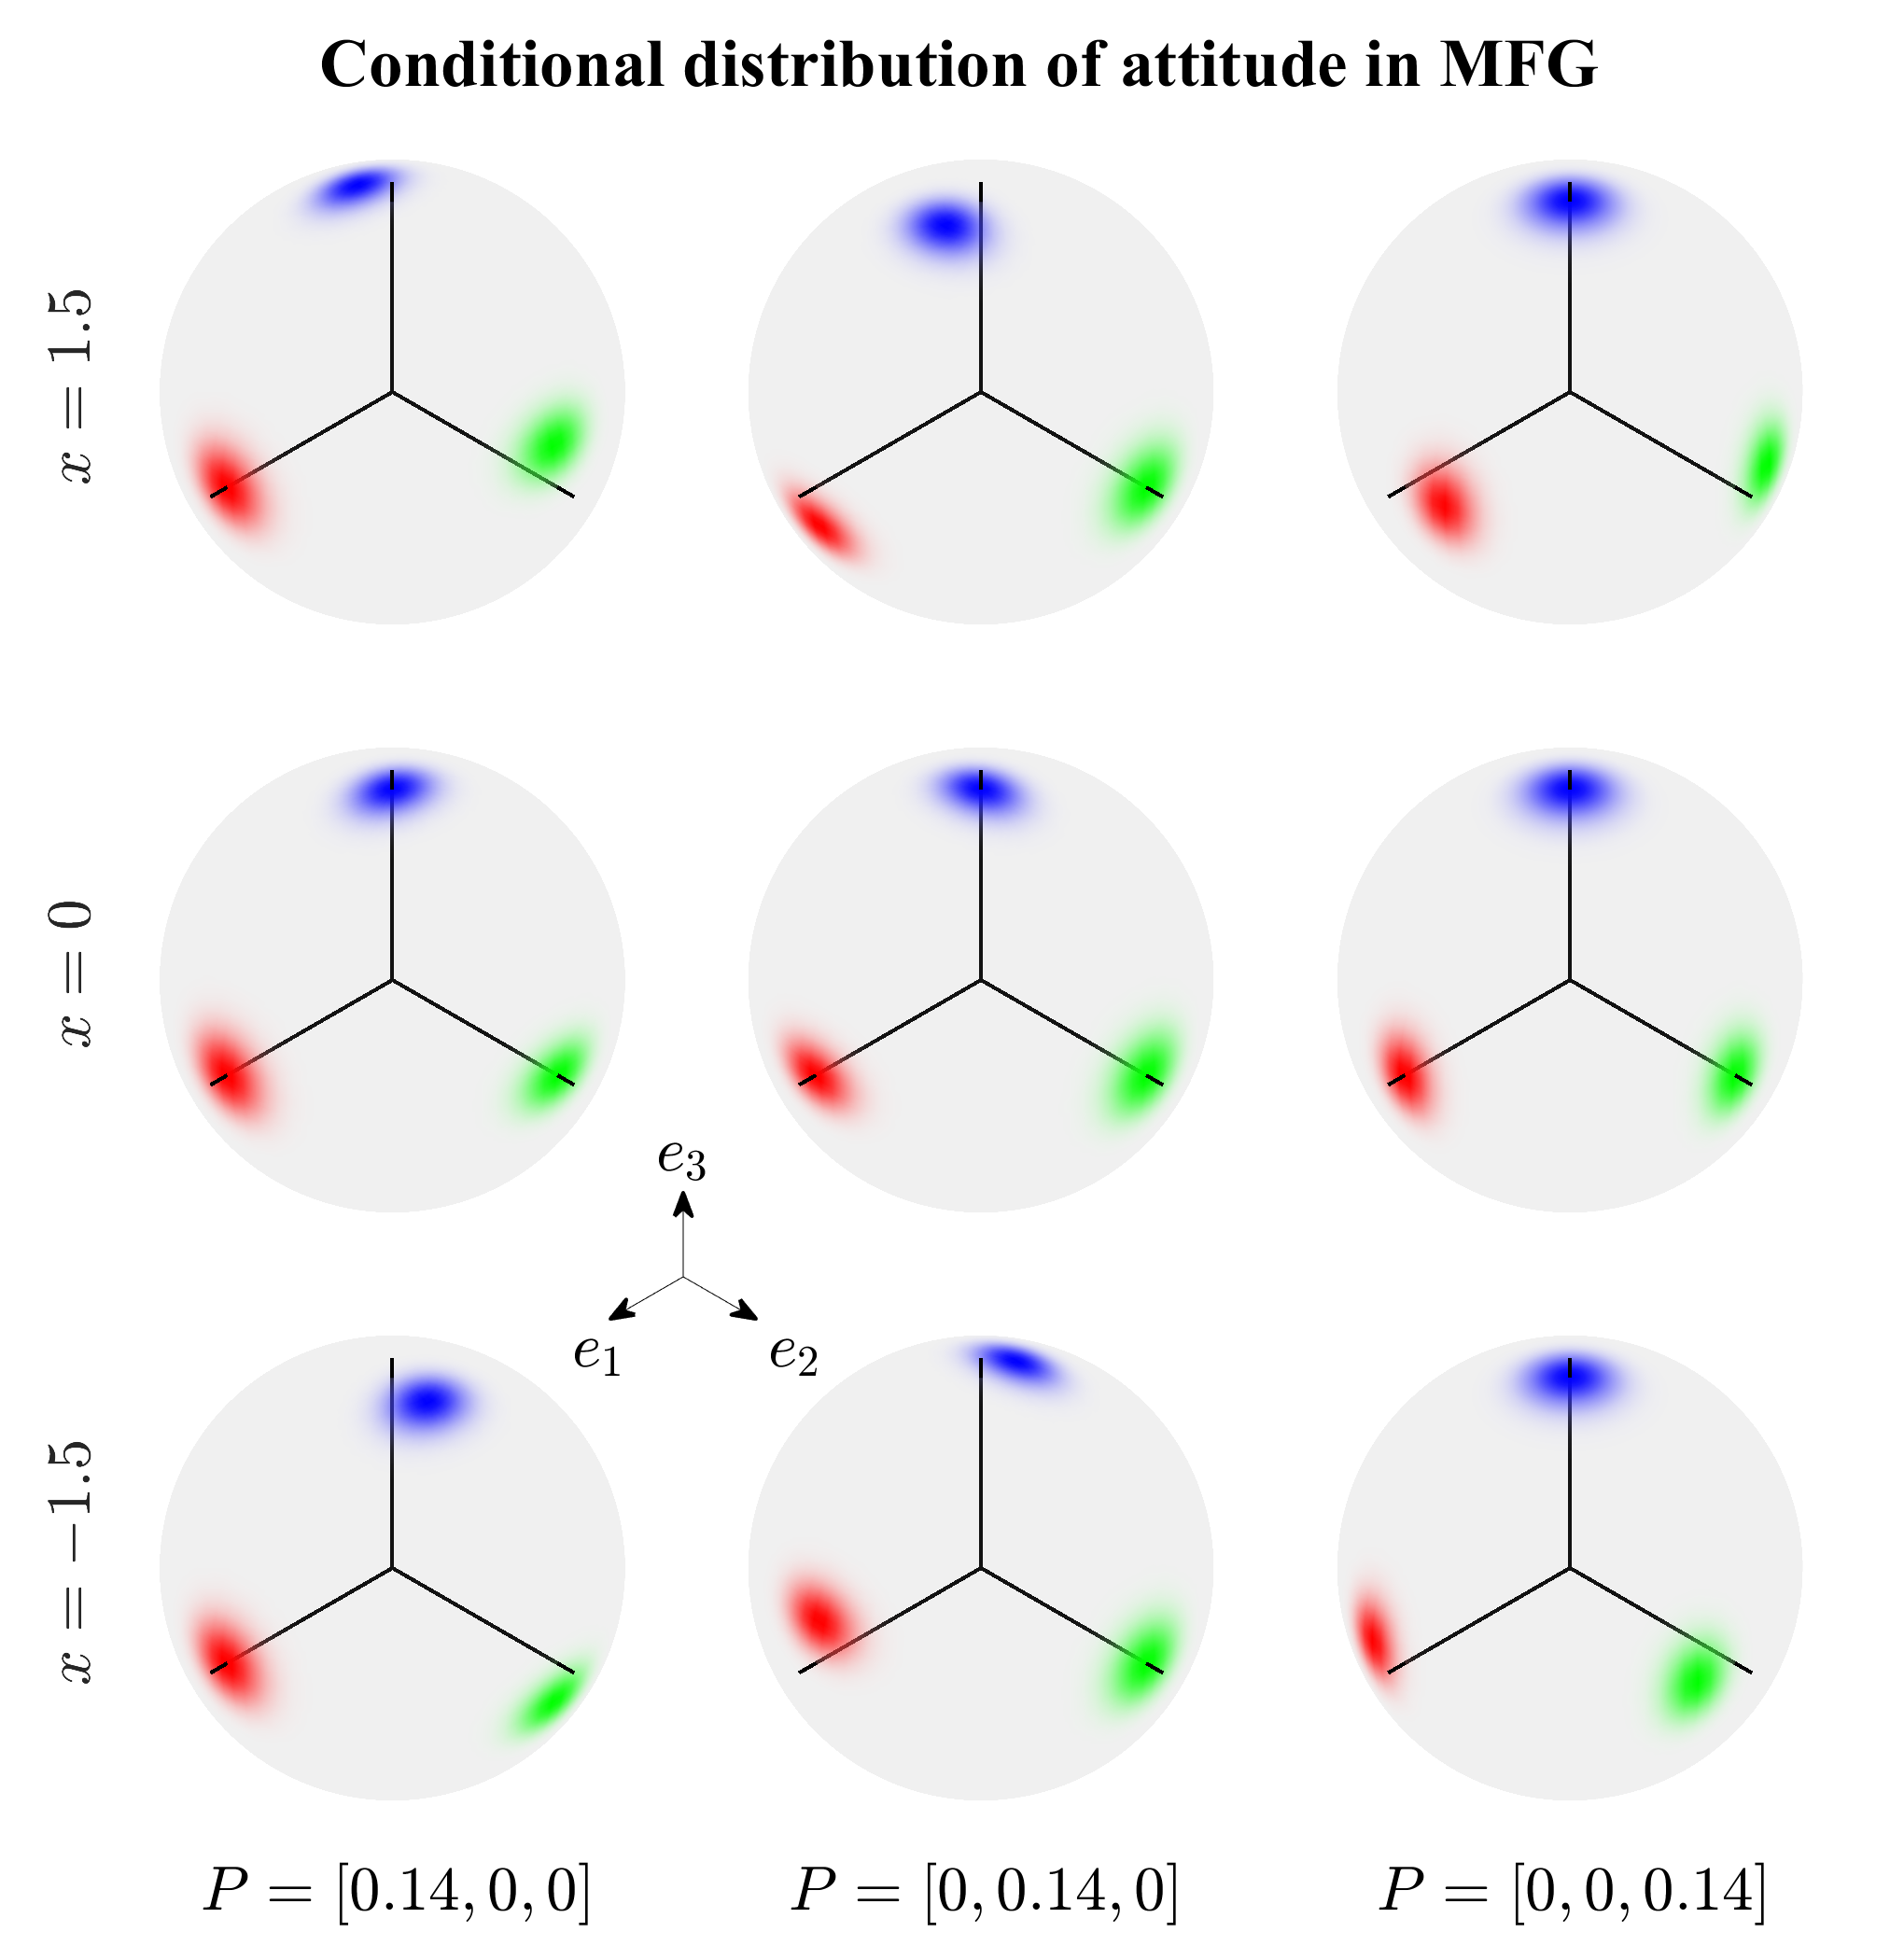
\includegraphics[scale=0.75]{MFG-correlation}
	}
\end{frame}

\begin{frame}
	\frametitle{Difference Between MFGI and MFGB}
	
	\begin{itemize}
		\item Difference between MFGI and MFGB
		
		\only<1>{
			\begin{itemize}
				\item MFGI: $x$ is correlated with rotations expressed in the \Emph{inertial frame}.
				\begin{itemize}
					\item $R|x \approxsim \mathcal{MG}\left( \exp(\widehat{U\upsilon(x)})USV^T \right)$.
				\end{itemize}
				\item MFGB: $x$ is correlated with rotations expressed in the \Emph{body-fixed frame}.
				\begin{itemize}
					\item $R|x \approxsim \mathcal{MG}\left( USV^T \exp(\widehat{V\upsilon(x)}) \right)$.
				\end{itemize}
			\end{itemize}
		}
		
		\only<2>{
			\vspace{0.5cm}
			\centerline{
				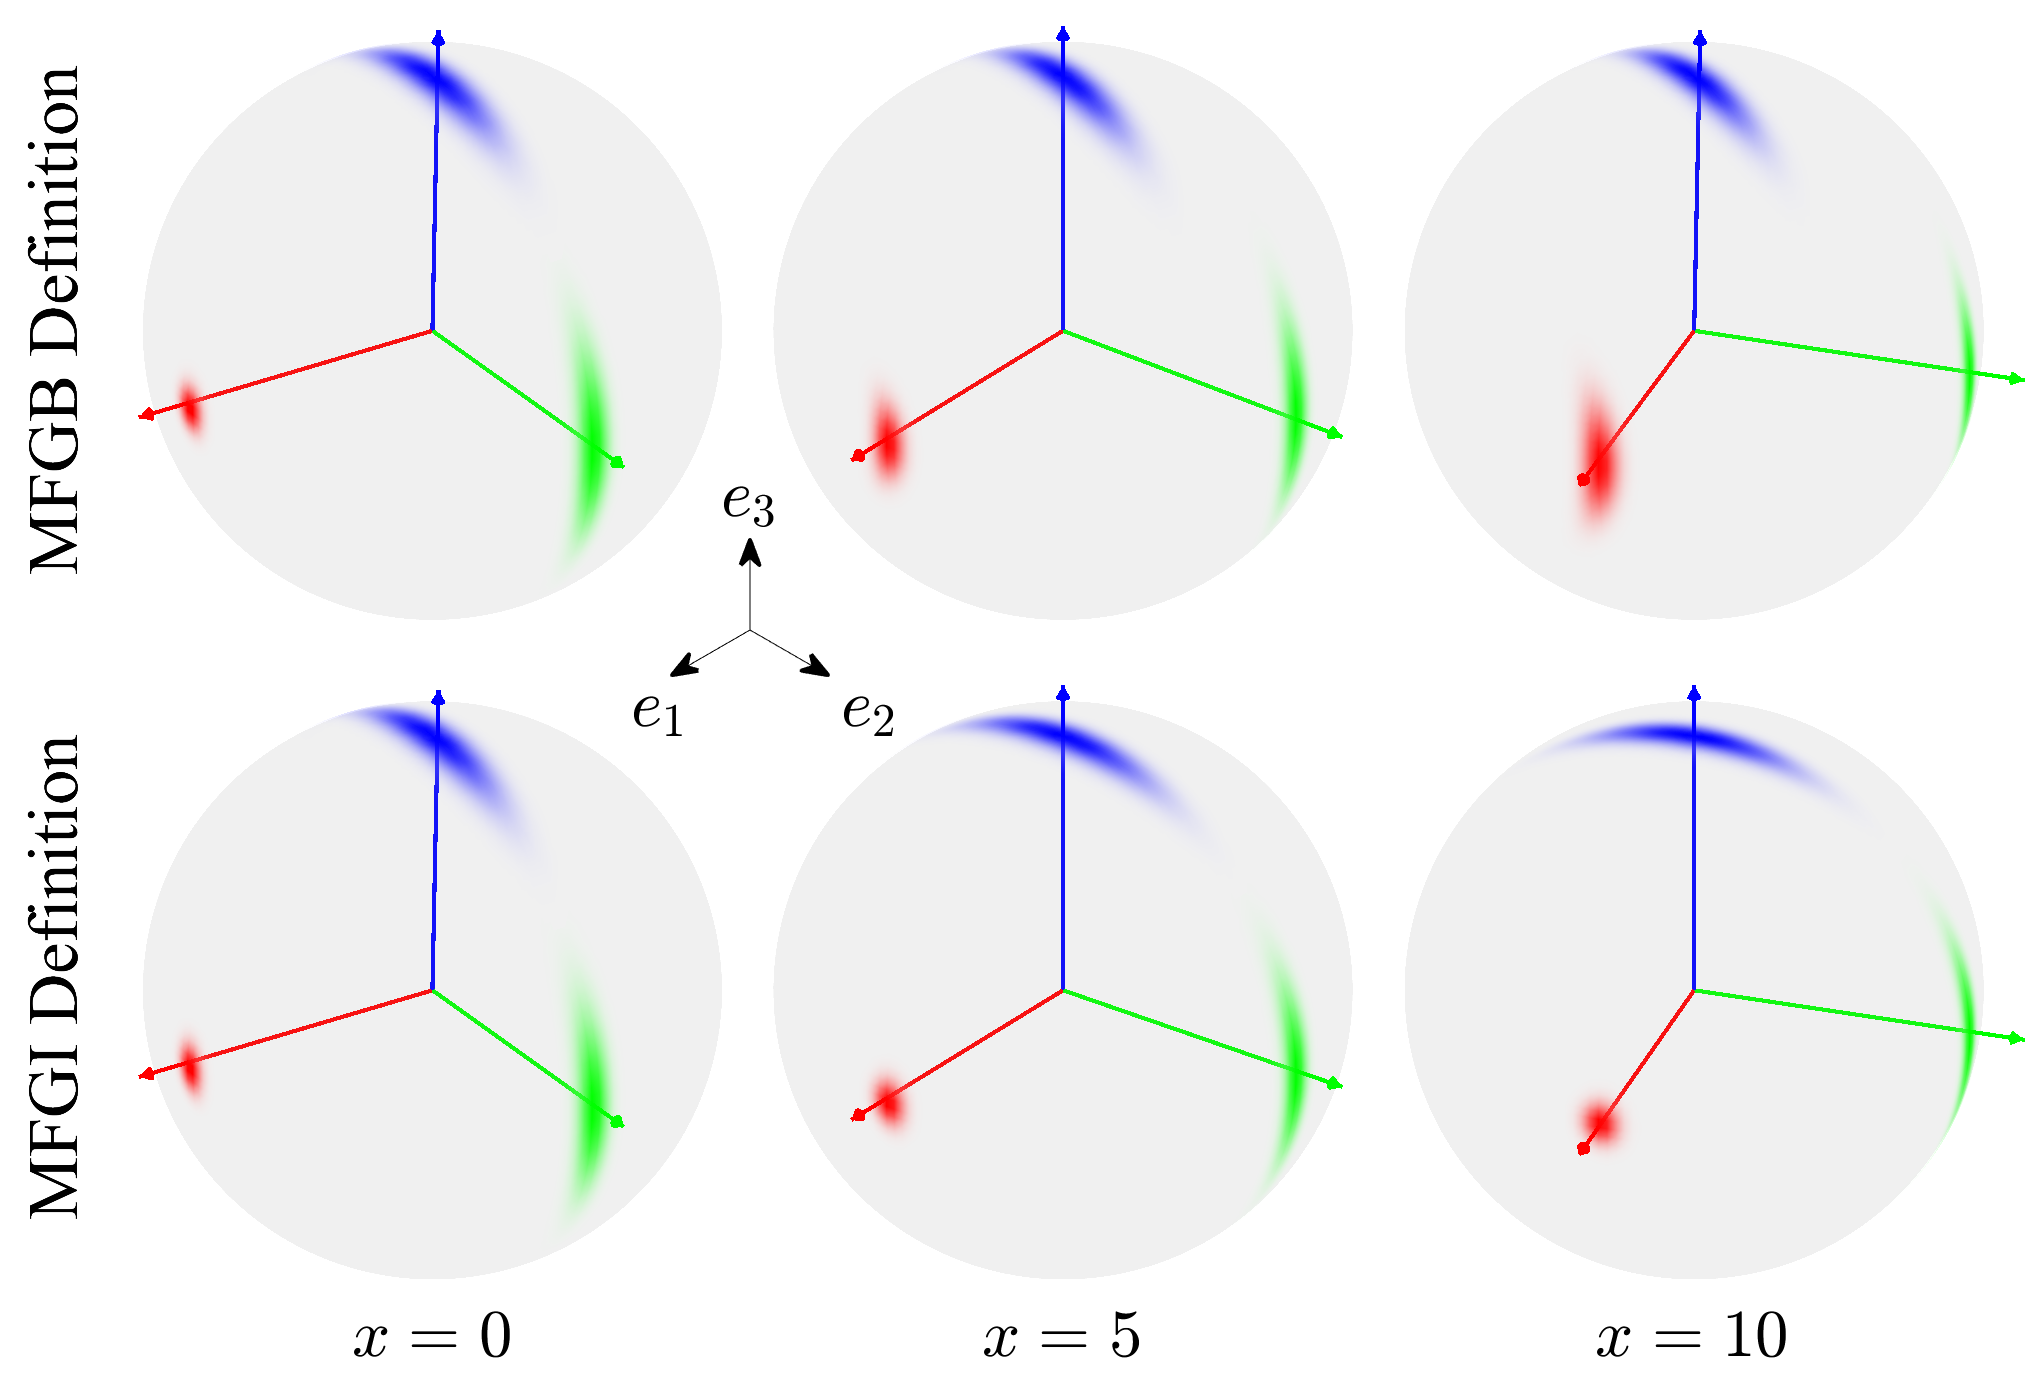
\includegraphics[scale=0.9]{MFG-MFGI-MFGB}
			}
		}
	\end{itemize}
\end{frame}

\begin{frame}
	\frametitle{Properties}
	
	\begin{itemize}
		\item Moments
		\begin{itemize}
			\item \makebox[1.1cm]{Attitude:} $\expect{R} = UDV^T$, $\expect{\nu_R} = 0$, $\expect{\nu_R\nu_R^T}_{ii} = s_j\expect{Q_{jj}} + s_k\expect{Q_{kk}}$ for $i\neq j\neq k$.
			\item Linear: $\expect{x} = \mu$, $\expect{xx^T} = \mu\mu^T + \Sigma - P(\tr{S}I-S)P^T + P\expect{v_Rv_R^T}P^T$.
			\item Correlation: $\expect{x\nu_R^T} = P\expect{\nu_R\nu_R^T}$.
		\end{itemize}
	
		\vspace{0.2cm}
		\item Maximum Likelihood Estimation for Parameters
		\begin{itemize}
			\item \Emph{Marginal} Likelihood for $R$: $U,S,V$.
			\begin{itemize}
				\item $UDV^T = \expect{R}$ is the proper SVD.
				\item Solve $S$ from $d_i = \frac{1}{c(S)} \frac{\partial c(S)}{\partial s_i}$ for $i=1,2,3$.
			\end{itemize}
		
			\item \Emph{Conditional} Likelihood for $x\lvert R$: $\mu,\Sigma,P$
			\begin{itemize}
				\item $P = \mathrm{cov}(x,\nu_R)\mathrm{cov}(\nu_R,\nu_R)^{-1}$.
				\item $\mu = \mathrm{E}[x]-P\mathrm{E}[\nu_R]$.
				\item $\Sigma = \mathrm{cov}(x,x)-P\mathrm{cov}(x,\nu_R)^T+P(\tr{S}I_{3\times 3}-S)P^T$.
			\end{itemize}
		
			\item The marginal-conditional MLE is an approximation to the full MLE.
			\item This closed form solution makes the calculation efficient,  thus \Emph{suitable for real time implementations}.
		\end{itemize}
	\end{itemize}
\end{frame}

\section{Attitude Estimation With MFG}

\begin{frame}
	\frametitle{Attitude Estimation}
	
	\begin{itemize}
		\item Attitude Observability with Single Direction Measurements
		\item Attitude Estimation Based on MFG
	\end{itemize}
\end{frame}

\subsection{Attitude Observability with Single Direction Measurements}

\begin{frame}
	\frametitle{Problem Formulation}
	
	\begin{itemize}
		\item Attitude kinematics
		
		\centerline{
			\begin{beamercolorbox}[wd=10cm,sep=0.0cm,center,rounded=true,shadow=true]{numerical}
				\small
				\vspace{-0.4cm}
				\begin{subequations}
					\begin{align} \small
						\frac{\diff{R}(t)}{\diff{t}} &= R(t)\hat{\Omega}(t) \\
						\frac{\diff{R}(t)}{\diff{t}} &= \hat{\omega}(t)R(t)
					\end{align}
				\end{subequations}
				\vspace{-0.4cm}
			\end{beamercolorbox}
		}
		
		\begin{itemize}
			\item $\Omega(t)$: angular velocity measured in body-fixed frame.
			\item $\omega(t)$: angular velocity measured in inertial frame.
		\end{itemize}
		
		\vspace{0.2cm}
		\item Single direction measurements
		
		\centerline{
			\begin{beamercolorbox}[wd=10cm,sep=0.0cm,center,rounded=true,shadow=true]{numerical}
				\small
				\vspace{-0.4cm}
				\begin{subequations}
					\begin{align} \small
						x(t) &= R(t)^T a \\
						y(t) &= R(t) b
					\end{align}
				\end{subequations}
				\vspace{-0.5cm}
			\end{beamercolorbox}
		}
		
		\begin{itemize}
			\item $a$: reference vector in inertial frame, e.g., the direction of magnetic field, or towards a star.
			$x(t)$: measurement in body-fixed frame.
			
			\item $b$: reference vector in body-fixed frame, e.g., the direction towards solar panel from the center.
			$y(t)$: measurement in inertial frame.
		\end{itemize}
	\end{itemize}
\end{frame}

\begin{frame}
	\frametitle{Attitude Observability}
	
	\centerline{
		\begin{beamercolorbox}[wd=10cm,sep=0.0cm,center,rounded=true,shadow=true]{numerical}
			\small
			\vspace{-0.4cm}
			\setcounter{equation}{0}
			\begin{subequations}
				\begin{align} \small
					\frac{\diff{R}(t)}{\diff{t}} &= R(t)\hat{\Omega}(t) \\
					\frac{\diff{R}(t)}{\diff{t}} &= \hat{\omega}(t)R(t)
				\end{align}
			\end{subequations}
			\vspace{-0.4cm}
		\end{beamercolorbox}
	}
	
	\centerline{
		\begin{beamercolorbox}[wd=10cm,sep=0.0cm,center,rounded=true,shadow=true]{numerical}
			\small
			\vspace{-0.4cm}
			\begin{subequations}
				\begin{align} \small
					x(t) &= R(t)^T a \\
					y(t) &= R(t) b
				\end{align}
			\end{subequations}
			\vspace{-0.5cm}
		\end{beamercolorbox}
	}
	
	\vspace{0.5cm}

	\begin{table}
		\centering
		\begin{tabular}{l|cc}
			\diagbox[width=10em]{ref. vec.}{ang. vel.} & \makecell{body-fixed frame \\ (1a)} & \makecell{inertial frame \\ (1b)} \\ \hline
			body-fixed frame (2b) & \color{red} observable & unobservable \\
			inertial frame (2a) & unobservable & \color{red} observable
		\end{tabular}
	\end{table}	
\end{frame}

\begin{frame}
	\frametitle{Uncertainty Propagation}
	
	\begin{itemize}
		\item Angular velocity in body-fixed frame: $\tfrac{\diff{R}(t)}{\diff{t}} = R(t)\hat{\Omega}(t)$
		\begin{itemize}
			\item The uncertainty is rotated in the body-fixed frame, but is unchanged in the inertial frame.
		\end{itemize}
		
		\centerline{
			\begin{tikzpicture}
				\node[opacity=1.0,outer sep=0pt,inner sep=0pt] at (-3.0,0) {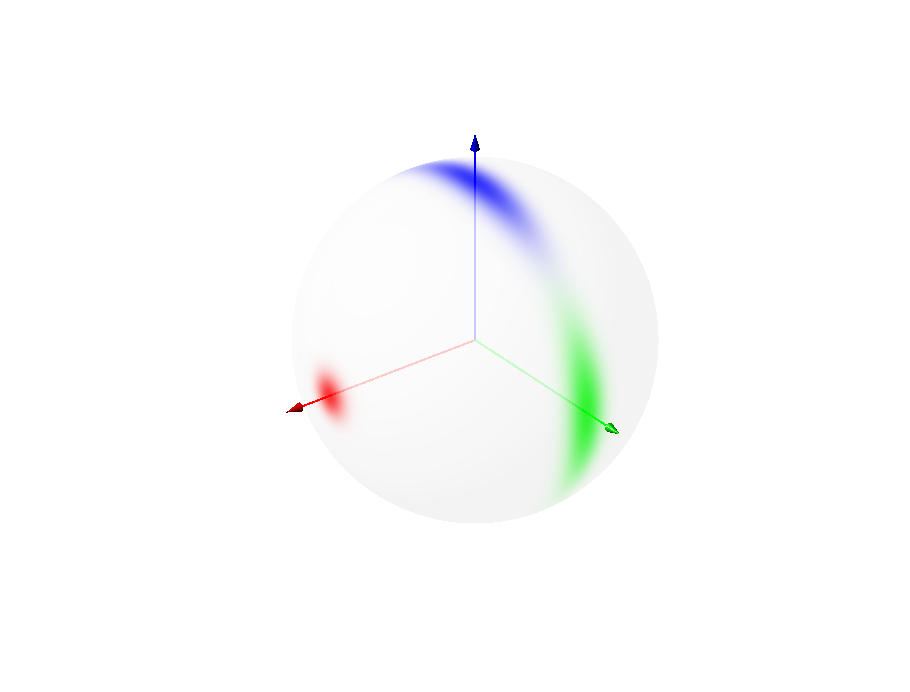
\includegraphics[width=0.2\columnwidth, trim=100 60 100 40, clip]{prop_L_1}};
				\node[opacity=1.0,outer sep=0pt,inner sep=0pt] at (0,0.1) {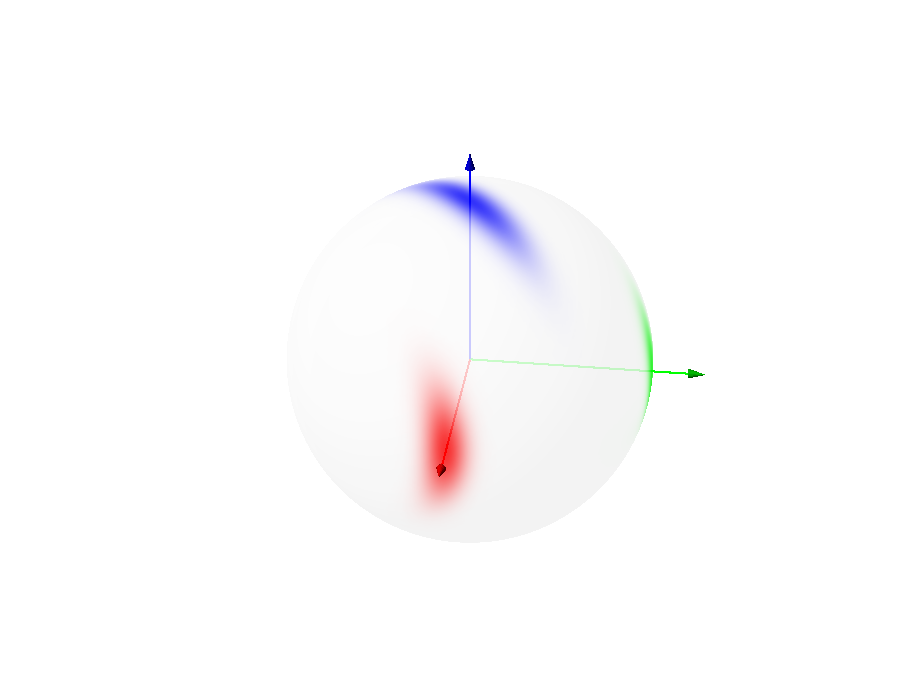
\includegraphics[width=0.2\columnwidth, trim=100 60 100 40, clip]{prop_L_2}};
				\node[opacity=1.0,outer sep=0pt,inner sep=0pt] at (3.0,0.1) {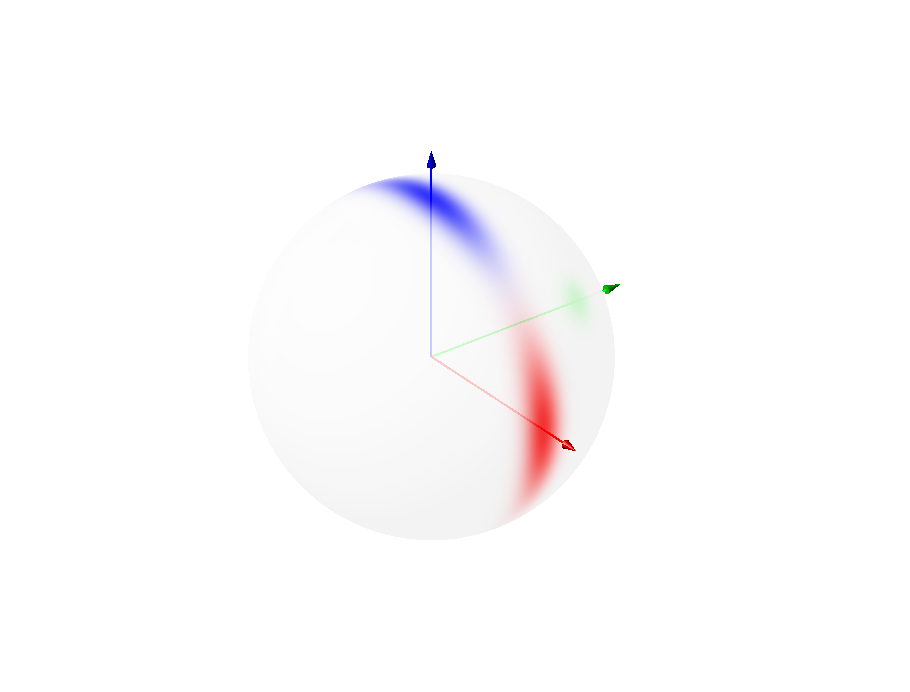
\includegraphics[width=0.2\columnwidth, trim=100 60 100 40, clip]{prop_L_3}};
				\node[opacity=1.0,outer sep=0pt,inner sep=0pt] at (-2.9,-1.1) {\scriptsize $t=0$s};
				\node[opacity=1.0,outer sep=0pt,inner sep=0pt] at (0.1,-1.1) {\scriptsize $t=0.5$s};
				\node[opacity=1.0,outer sep=0pt,inner sep=0pt] at (3.0,-1.1) {\scriptsize $t=1$s};
				
				\draw[arrows={-Triangle[angle=30:3pt]}] (-1.4,-0.6) -- ++(90:0.4);
				\draw[arrows={-Triangle[angle=30:3pt]}] (-1.4,-0.6) -- ++(-30:0.4);
				\draw[arrows={-Triangle[angle=30:3pt]}] (-1.4,-0.6) -- ++(210:0.4);
				\node at (-1.75,-0.95) {\tiny $\mathbf{e}_1$};
				\node at (-0.95,-0.95) {\tiny $\mathbf{e}_2$};
				\node at (-1.37,-0.12) {\tiny $\mathbf{e}_3$};
			\end{tikzpicture}
		}
		
		\vspace{0.3cm}
		\item Angular velocity in inertial frame:  $\tfrac{\diff{R}(t)}{\diff{t}} = \hat{\omega}(t)R(t)$
		\begin{itemize}
			\item The uncertainty is unchanged in the body-fixed frame, but is rotated in the inertial frame.
		\end{itemize}
		
		\centerline{
			\begin{tikzpicture}
				\node[opacity=1.0,outer sep=0pt,inner sep=0pt] at (-3.0,0) {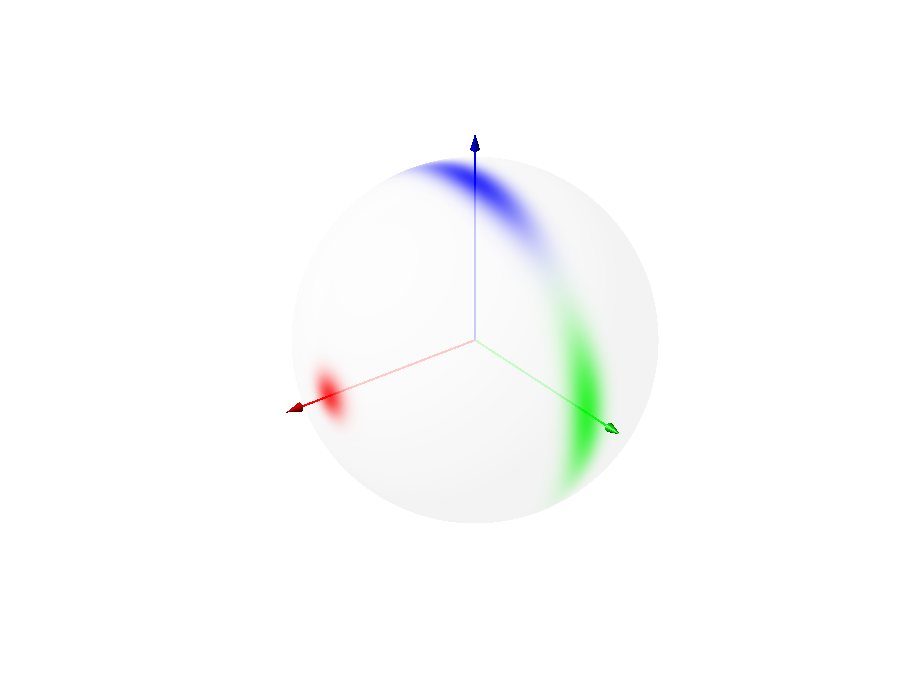
\includegraphics[width=0.2\columnwidth, trim=100 60 100 40, clip]{prop_R_1}};
				\node[opacity=1.0,outer sep=0pt,inner sep=0pt] at (0,0.1) {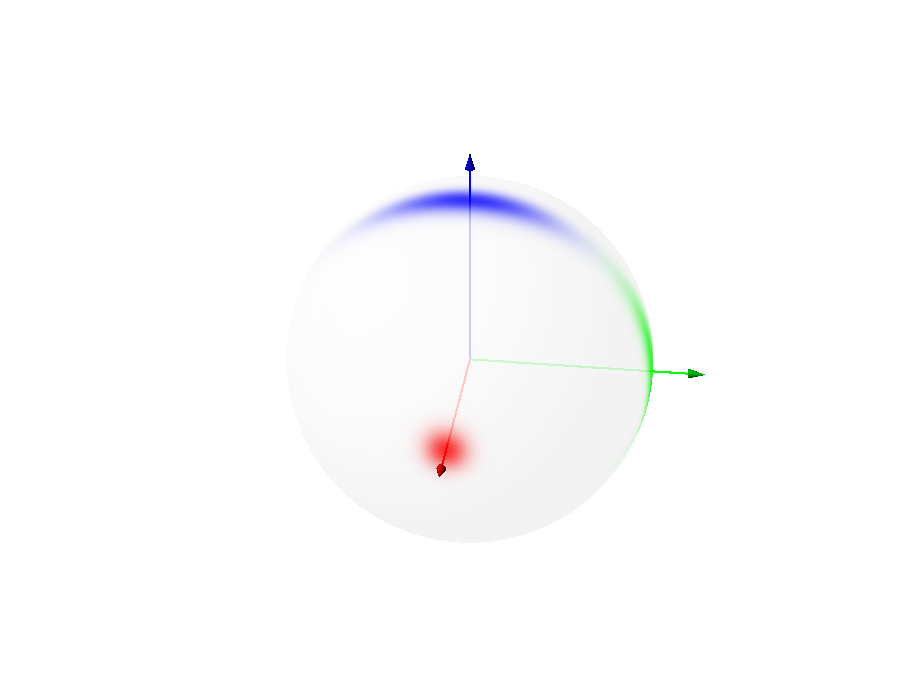
\includegraphics[width=0.2\columnwidth, trim=100 60 100 40, clip]{prop_R_2}};
				\node[opacity=1.0,outer sep=0pt,inner sep=0pt] at (3.0,0.1) {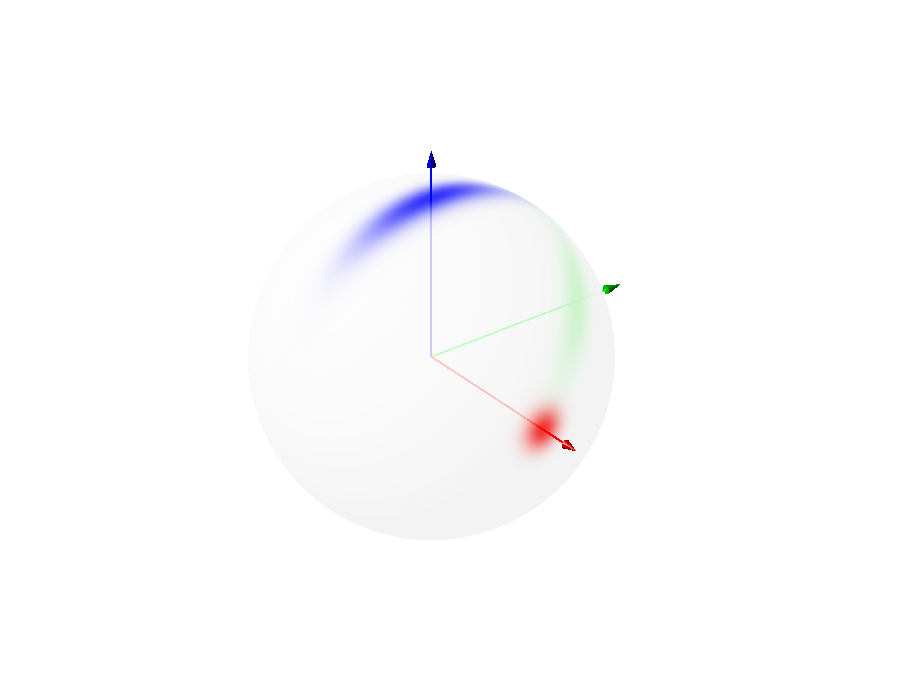
\includegraphics[width=0.2\columnwidth, trim=100 60 100 40, clip]{prop_R_3}};
				\node[opacity=1.0,outer sep=0pt,inner sep=0pt] at (-2.9,-1.1) {\scriptsize $t=0$s};
				\node[opacity=1.0,outer sep=0pt,inner sep=0pt] at (0.1,-1.1) {\scriptsize $t=0.5$s};
				\node[opacity=1.0,outer sep=0pt,inner sep=0pt] at (3.0,-1.1) {\scriptsize $t=1$s};
				
				\draw[arrows={-Triangle[angle=30:3pt]}] (-1.4,-0.6) -- ++(90:0.4);
				\draw[arrows={-Triangle[angle=30:3pt]}] (-1.4,-0.6) -- ++(-30:0.4);
				\draw[arrows={-Triangle[angle=30:3pt]}] (-1.4,-0.6) -- ++(210:0.4);
				\node at (-1.75,-0.95) {\tiny $\mathbf{e}_1$};
				\node at (-0.95,-0.95) {\tiny $\mathbf{e}_2$};
				\node at (-1.37,-0.12) {\tiny $\mathbf{e}_3$};
			\end{tikzpicture}
		}
	\end{itemize}
\end{frame}

\begin{frame}
	\frametitle{Correction From Direction Measurements}
	\begin{itemize}
		\item Reference direction in inertial frame: $x(t) = R(t)^Ta$
		\begin{itemize}
			\item Non-informative along direction $a$; $a$ is fixed in inertial frame.
		\end{itemize}
		
		\centerline{
			\begin{tikzpicture}
				\node[opacity=1.0,outer sep=0pt,inner sep=0pt] at (-3.0,0) {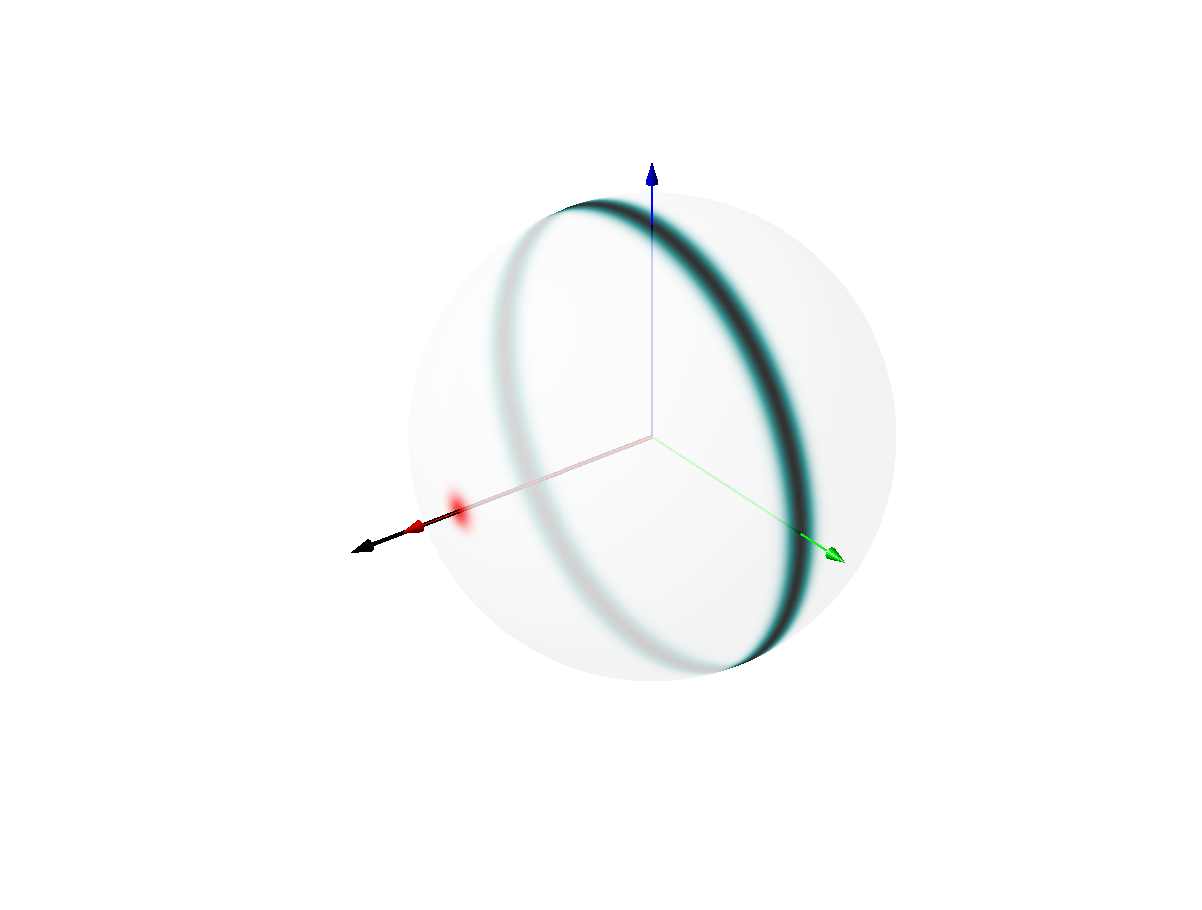
\includegraphics[width=0.2\columnwidth, trim=100 60 100 40, clip]{mea_I_1}};
				\node[opacity=1.0,outer sep=0pt,inner sep=0pt] at (0,0.1) {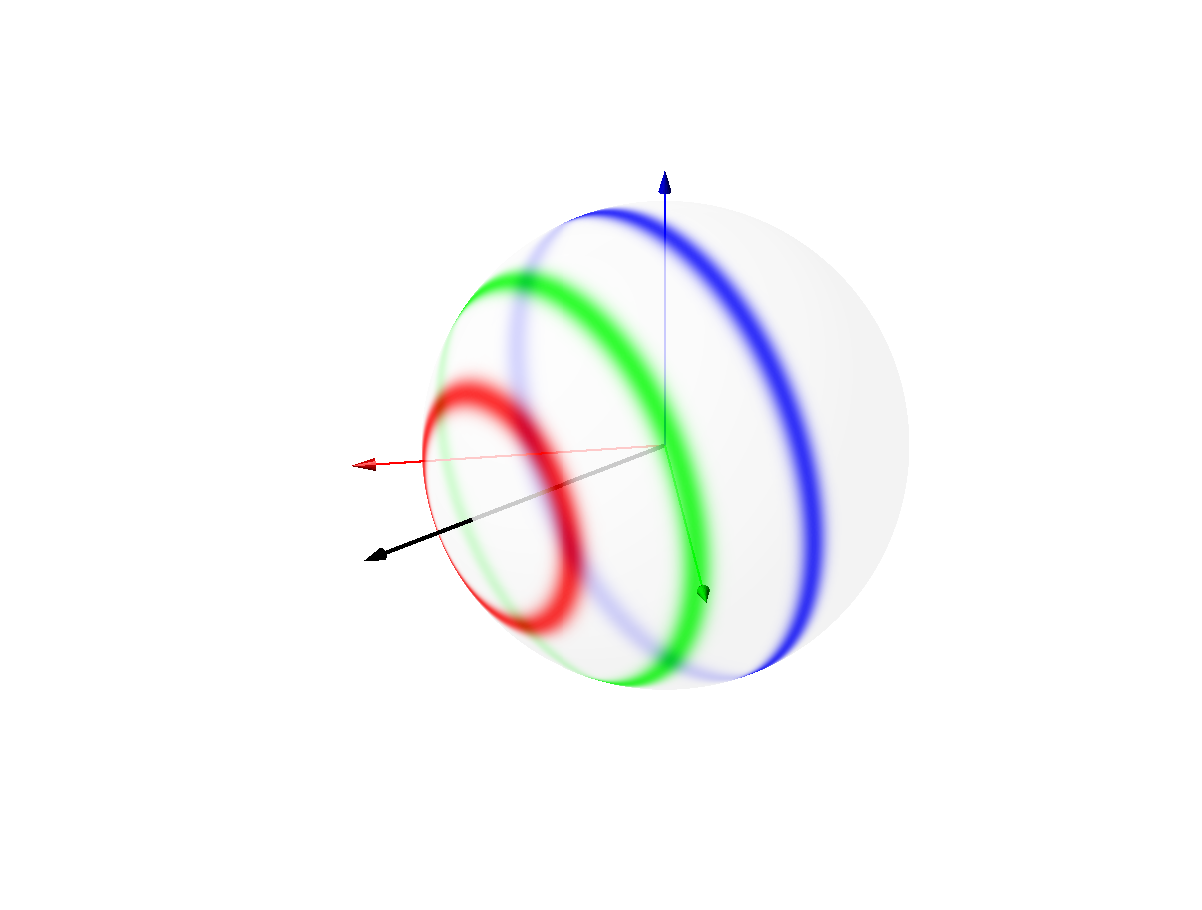
\includegraphics[width=0.2\columnwidth, trim=100 60 100 40, clip]{mea_I_2}};
				\node[opacity=1.0,outer sep=0pt,inner sep=0pt] at (3.0,0.1) {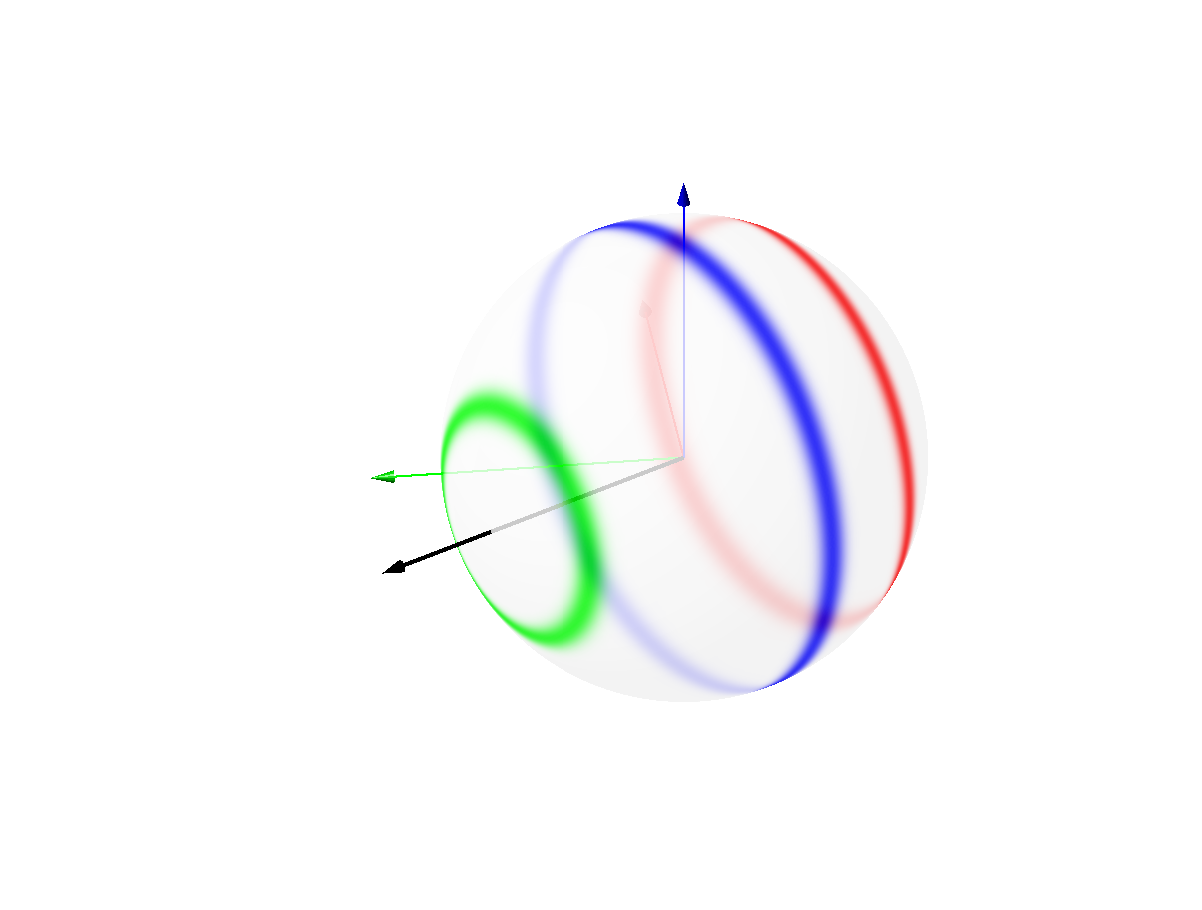
\includegraphics[width=0.2\columnwidth, trim=100 60 100 40, clip]{mea_I_3}};
				\node[opacity=1.0,outer sep=0pt,inner sep=0pt] at (-2.8,-1.1) {\scriptsize $x=e_1$};
				\node[opacity=1.0,outer sep=0pt,inner sep=0pt] at (0.2,-1.1) {\scriptsize $x=\tfrac{\sqrt{3}}{2}e_1 + \tfrac{1}{2}e_2$};
				\node[opacity=1.0,outer sep=0pt,inner sep=0pt] at (3.3,-1.1) {\scriptsize $x=-\tfrac{1}{2}e_1 + \tfrac{\sqrt{3}}{2}e_2$};
				
				\draw[arrows={-Triangle[angle=30:3pt]}] (-1.4,-0.6) -- ++(90:0.4);
				\draw[arrows={-Triangle[angle=30:3pt]}] (-1.4,-0.6) -- ++(-30:0.4);
				\draw[arrows={-Triangle[angle=30:3pt]}] (-1.4,-0.6) -- ++(210:0.4);
				\node at (-1.75,-0.95) {\tiny $\mathbf{e}_1$};
				\node at (-0.95,-0.95) {\tiny $\mathbf{e}_2$};
				\node at (-1.37,-0.12) {\tiny $\mathbf{e}_3$};
			\end{tikzpicture}
		}
		
		\vspace{0.3cm}
		\item Reference direction in body-fixed frame: $y(t) = R(t)b$
		\begin{itemize}
			\item Non-informative along direction $b$; $b$ is fixed in body-fixed frame.
		\end{itemize}
		
		\centerline{
			\begin{tikzpicture}
				\node[opacity=1.0,outer sep=0pt,inner sep=0pt] at (-3.0,0) {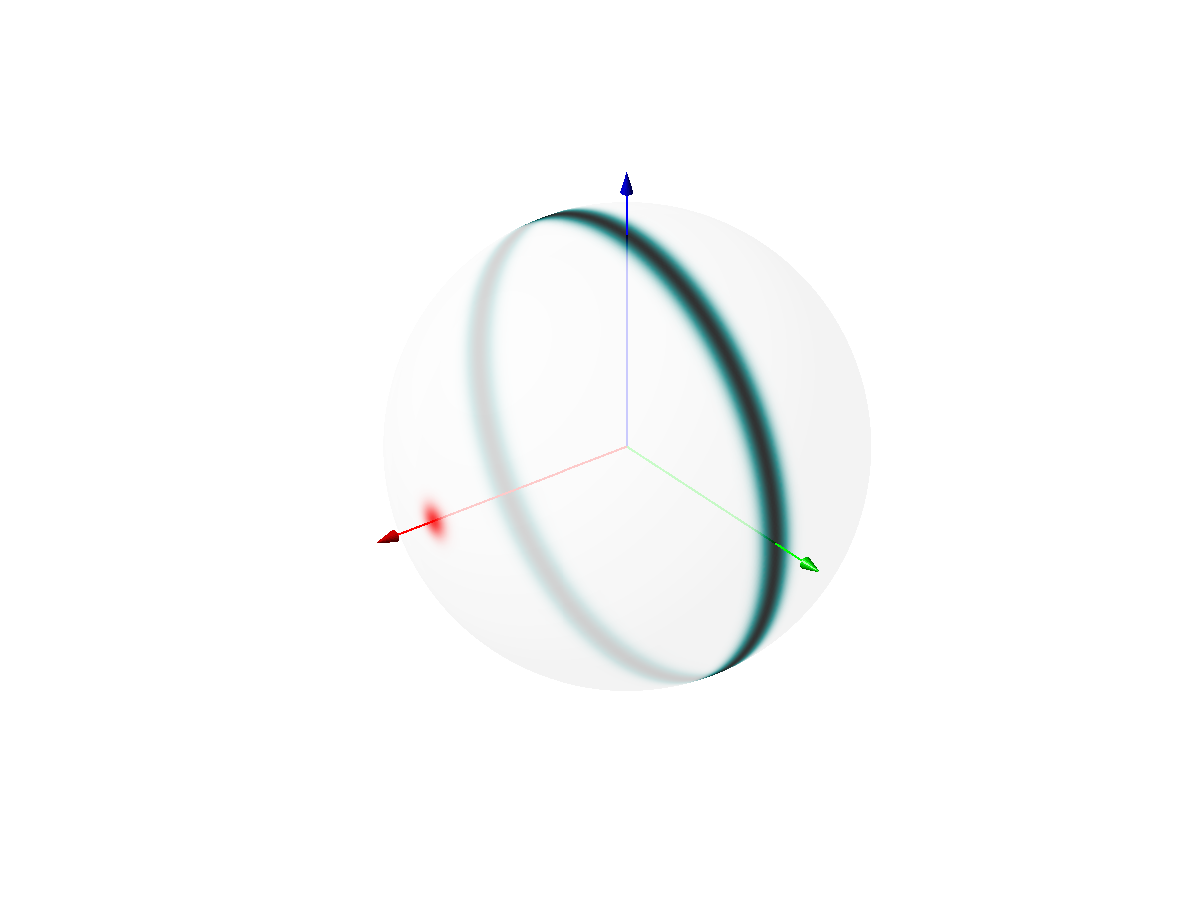
\includegraphics[width=0.2\columnwidth, trim=100 60 100 40, clip]{mea_B_1}};
				\node[opacity=1.0,outer sep=0pt,inner sep=0pt] at (0.0,0.1) {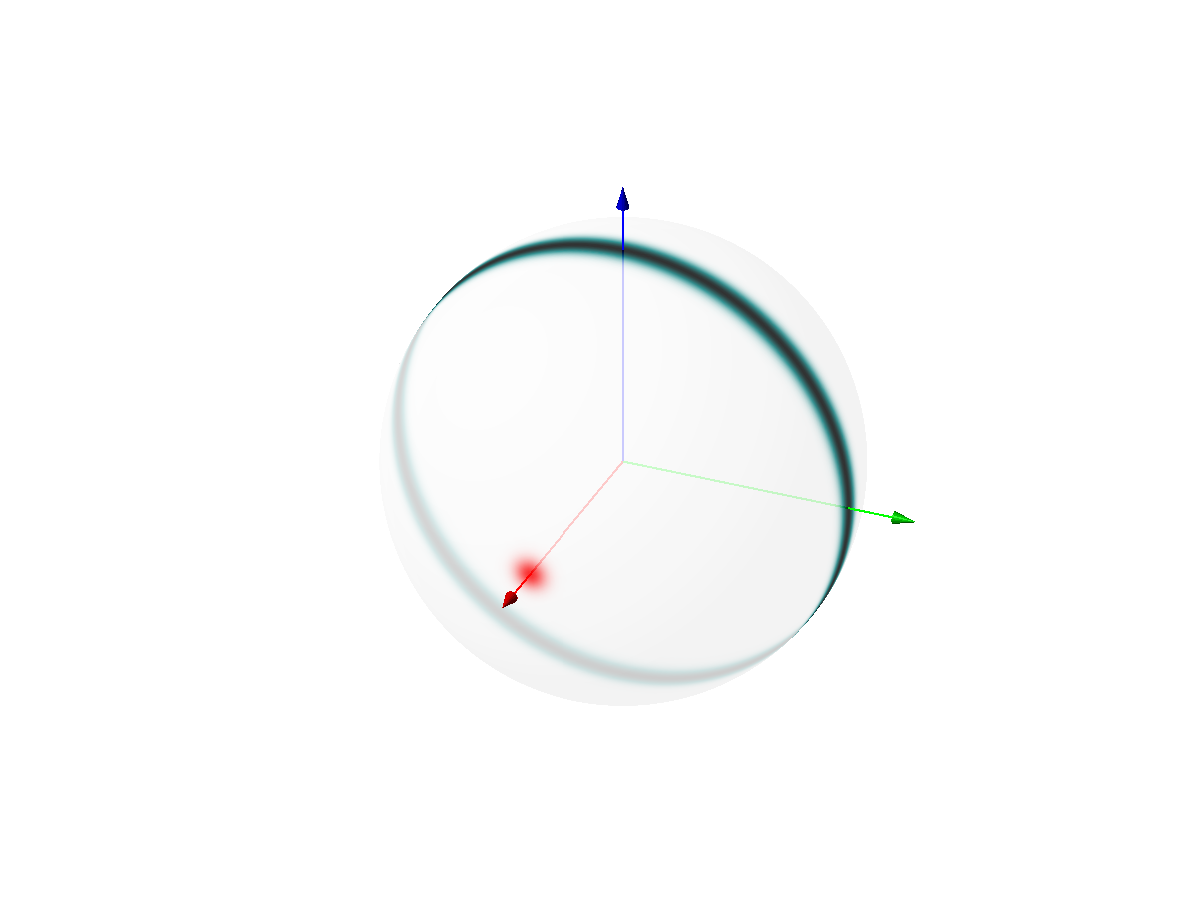
\includegraphics[width=0.2\columnwidth, trim=100 60 100 40, clip]{mea_B_2}};
				\node[opacity=1.0,outer sep=0pt,inner sep=0pt] at (3.0,0.1) {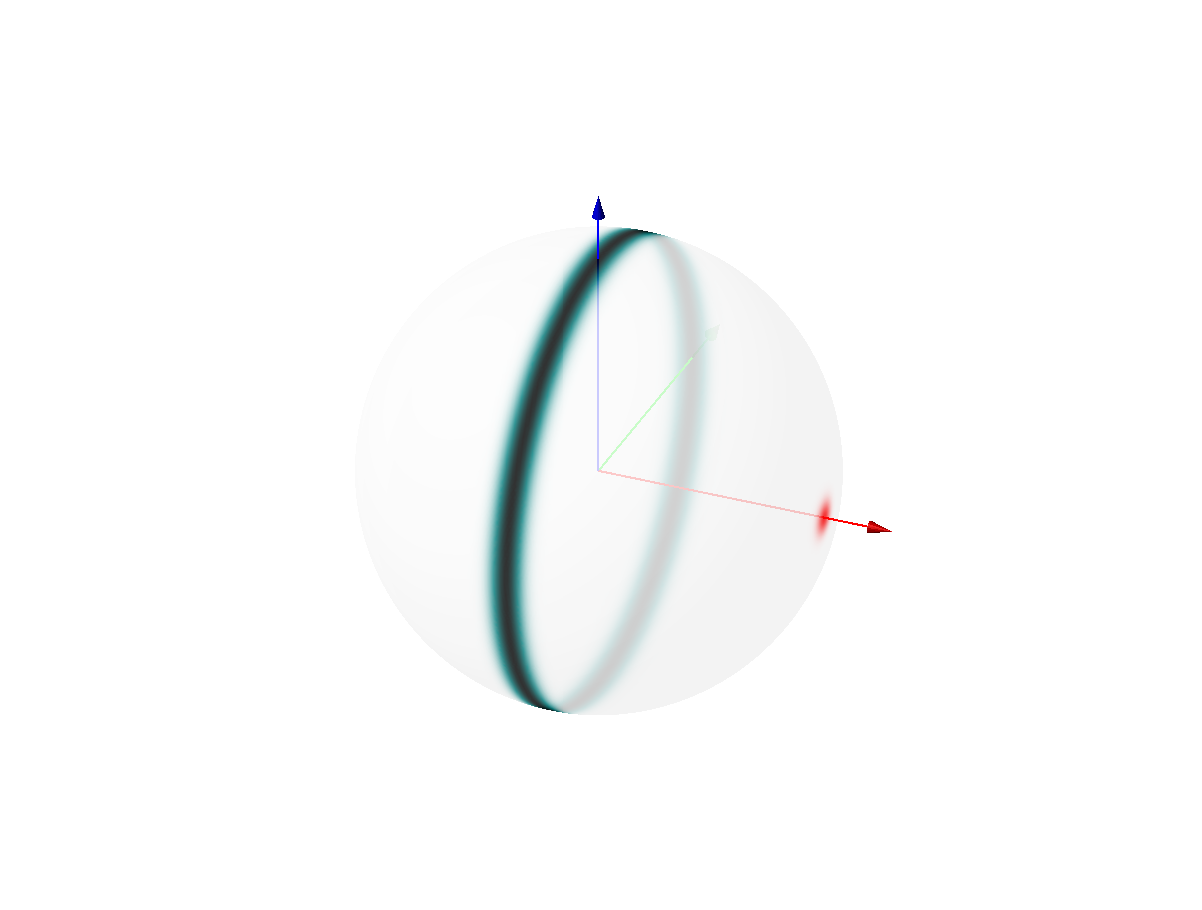
\includegraphics[width=0.2\columnwidth, trim=100 60 100 40, clip]{mea_B_3}};
				\node[opacity=1.0,outer sep=0pt,inner sep=0pt] at (-2.8,-1.1) {\scriptsize $y=e_1$};
				\node[opacity=1.0,outer sep=0pt,inner sep=0pt] at (0.2,-1.1) {\scriptsize $y=\tfrac{\sqrt{3}}{2}e_1 + \tfrac{1}{2}e_2$};
				\node[opacity=1.0,outer sep=0pt,inner sep=0pt] at (3.3,-1.1) {\scriptsize $y=-\tfrac{1}{2}e_1 + \tfrac{\sqrt{3}}{2}e_2$};
				
				\draw[arrows={-Triangle[angle=30:3pt]}] (-1.4,-0.6) -- ++(90:0.4);
				\draw[arrows={-Triangle[angle=30:3pt]}] (-1.4,-0.6) -- ++(-30:0.4);
				\draw[arrows={-Triangle[angle=30:3pt]}] (-1.4,-0.6) -- ++(210:0.4);
				\node at (-1.75,-0.95) {\tiny $\mathbf{e}_1$};
				\node at (-0.95,-0.95) {\tiny $\mathbf{e}_2$};
				\node at (-1.37,-0.12) {\tiny $\mathbf{e}_3$};
			\end{tikzpicture}
		}
	\end{itemize}
\end{frame}

\begin{frame}
	\frametitle{Observability}
	
	\begin{itemize}
		\item Observable:
		\begin{itemize}
			\item Angular velocity in body-fixed frame: $\tfrac{\diff{R}(t)}{\diff{t}} = R(t)\hat{\Omega}(t)$
			\item Reference direction in body-fixed frame: $y(t) = R(t)b$
		\end{itemize}
		
		\begin{figure}
			\centerline{
				\subfigure{
					
\includegraphics[width=0.20\textwidth, trim=150 80 120 60, clip]{est_LB_F1_prior}
				} \hspace{-0.2cm}
				\subfigure{
					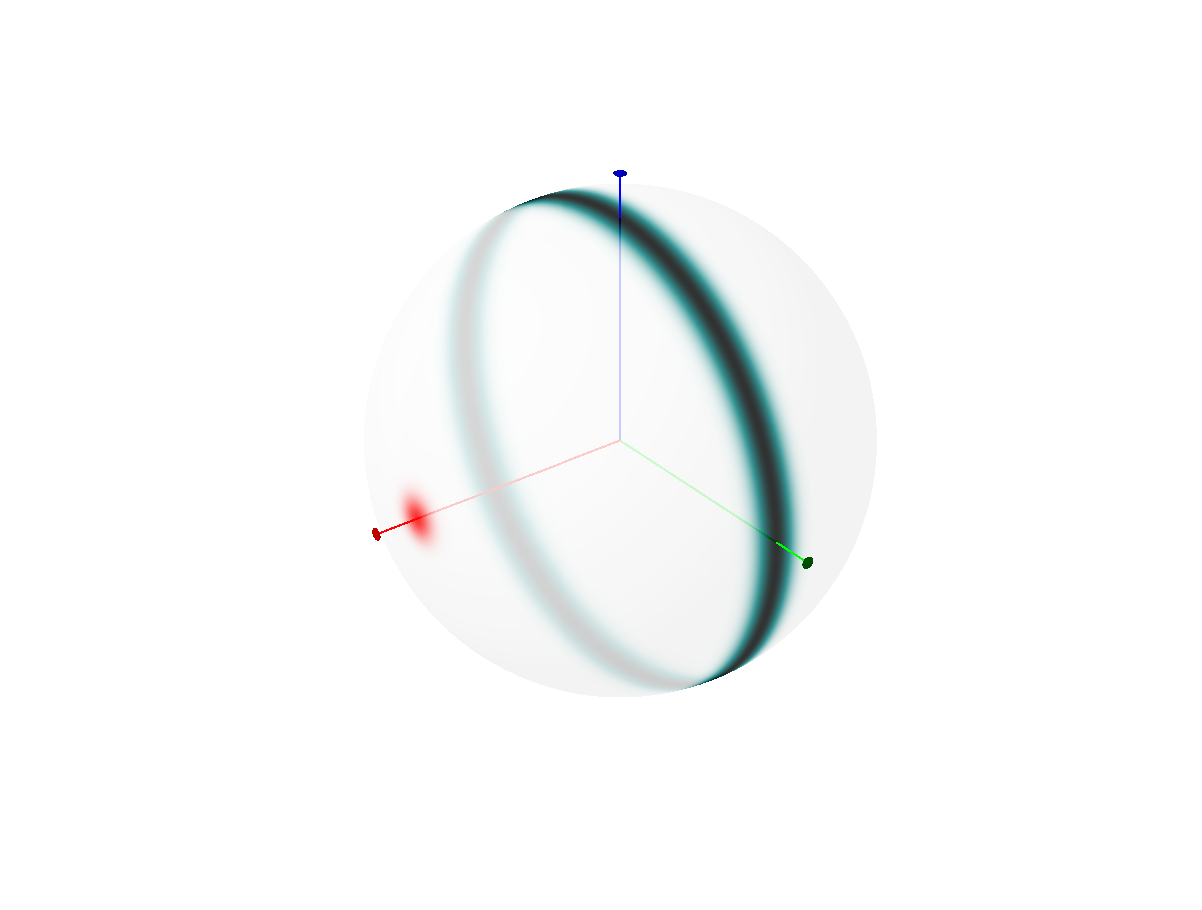
\includegraphics[width=0.20\textwidth, trim=150 80 120 60, clip]{est_LB_F1}
				} \hspace{-0.2cm}
				\subfigure{
					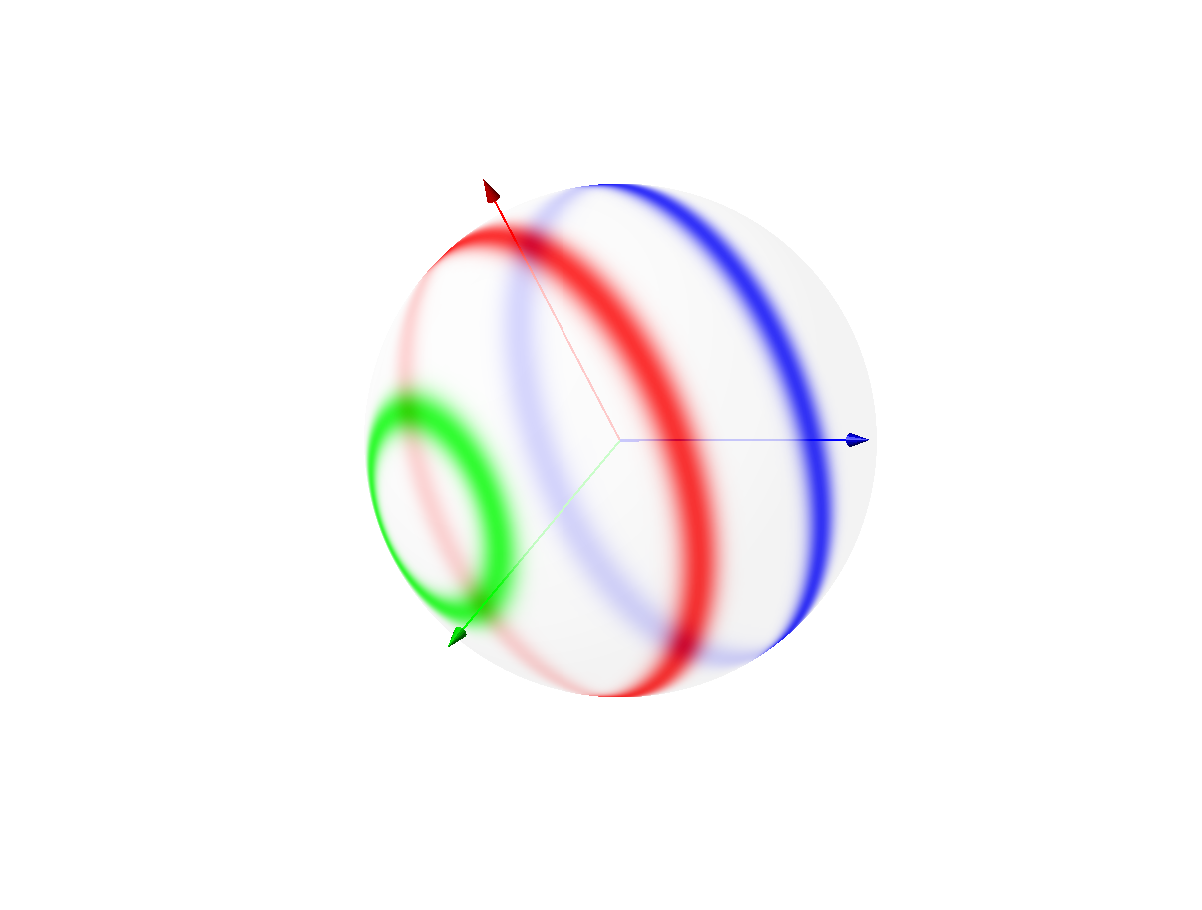
\includegraphics[width=0.20\textwidth, trim=150 80 120 60, clip]{est_LB_F5}
				} \hspace{-0.2cm}
				\subfigure{
					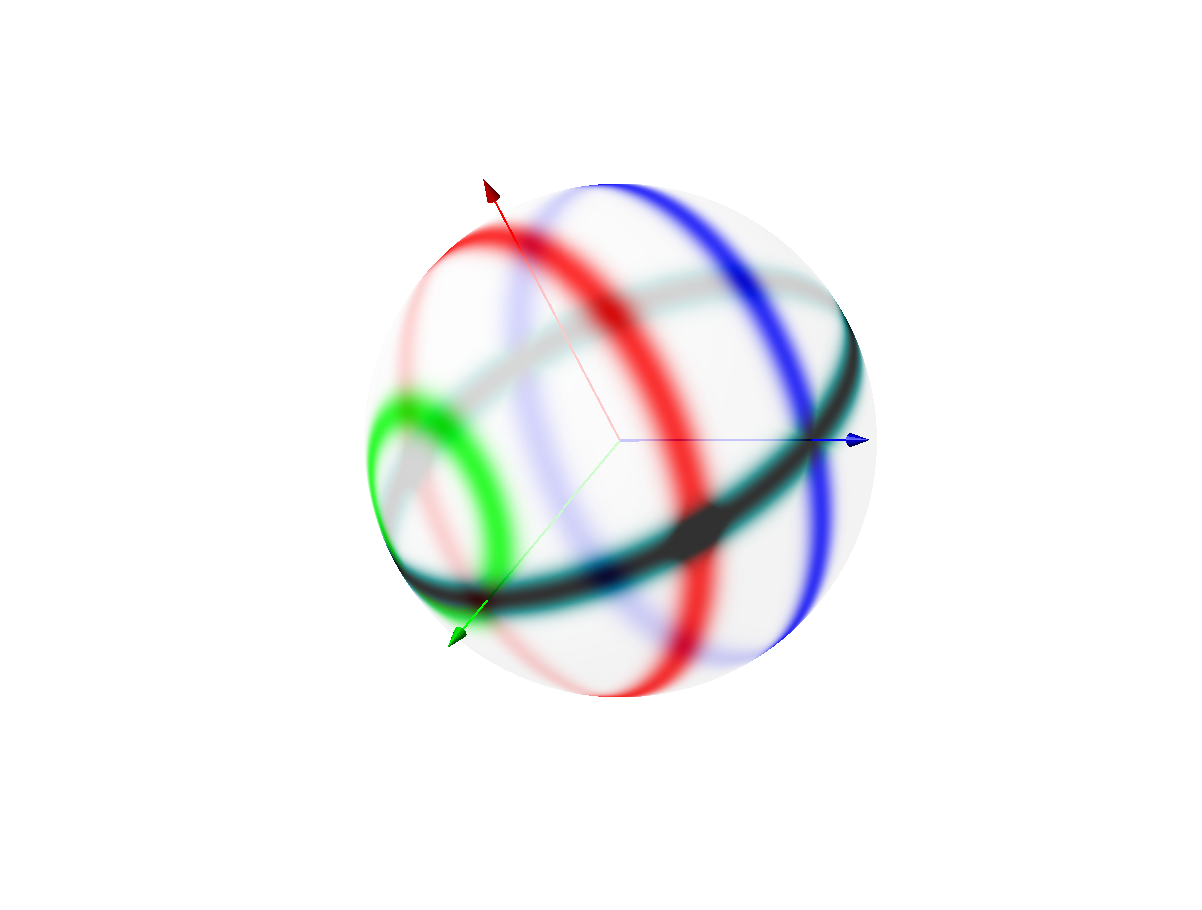
\includegraphics[width=0.20\textwidth, trim=150 80 120 60, clip]{est_LB_FN_mea}
				} \hspace{-0.2cm}
				\subfigure{
					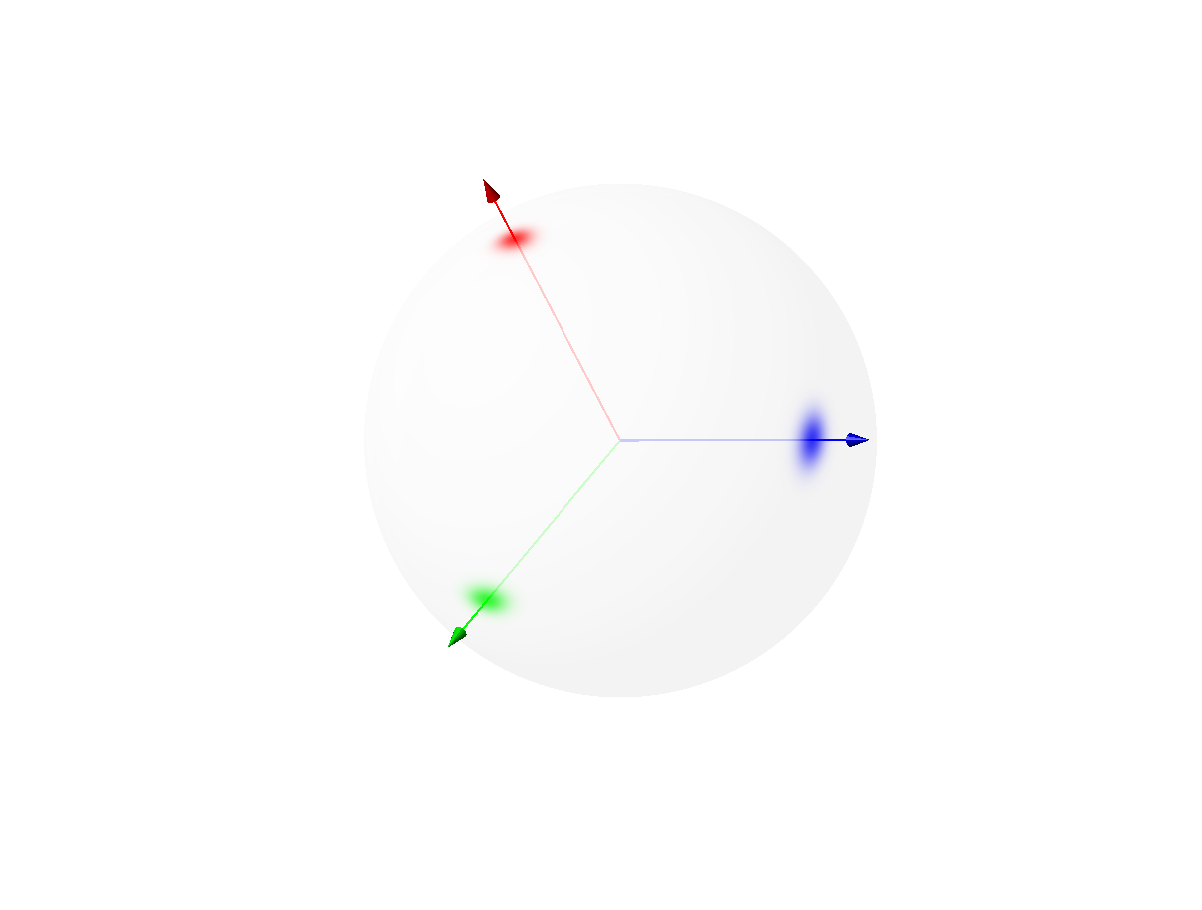
\includegraphics[width=0.20\textwidth, trim=150 80 120 60, clip]{est_LB_FN_post}
				}
			}
			\begin{tikzpicture}[overlay]
				\node at (-5.0,0.2) {\tiny Prior dist. at $t=0$};
				\node at (-2.65,0.2) {\tiny Posterior dist. at $t=0$};
				\node at (-0.3,0.2) {\tiny Propagated dist. at $t=1$};
				\node at (2.05,0.2) {\parbox{0.2\textwidth}{\tiny Propagated dist. overlapped \\ with measured dist. at $t=1$}};
				\node at (4.4,0.2) {\tiny Posterior dist. at $t=1$};
				
				\draw[arrows={-Triangle[angle=30:2pt]}] (-3.85,0.8) -- ++(90:0.3);
				\draw[arrows={-Triangle[angle=30:2pt]}] (-3.85,0.8) -- ++(-30:0.3);
				\draw[arrows={-Triangle[angle=30:2pt]}] (-3.85,0.8) -- ++(210:0.3);
				\node at (-4.15,0.5) {\tiny $\mathbf{e}_1$};
				\node at (-3.45,0.5) {\tiny $\mathbf{e}_2$};
				\node at (-3.82,1.23) {\tiny $\mathbf{e}_3$};
			\end{tikzpicture}
		\end{figure}
		
		\item Unobservable:
		\begin{itemize}
			\item Angular velocity in body-fixed frame: $\tfrac{\diff{R}(t)}{\diff{t}} = R(t)\hat{\Omega}(t)$
			\item Reference direction in inertial frame: $x(t) = R(t)^Ta$
		\end{itemize}
		
		\begin{figure}
			\centerline{
				\subfigure{
					
\includegraphics[width=0.20\textwidth, trim=115 60 95 20, clip]{est_LI_F1_prior}
				} \hspace{-0.2cm}
				\subfigure{
					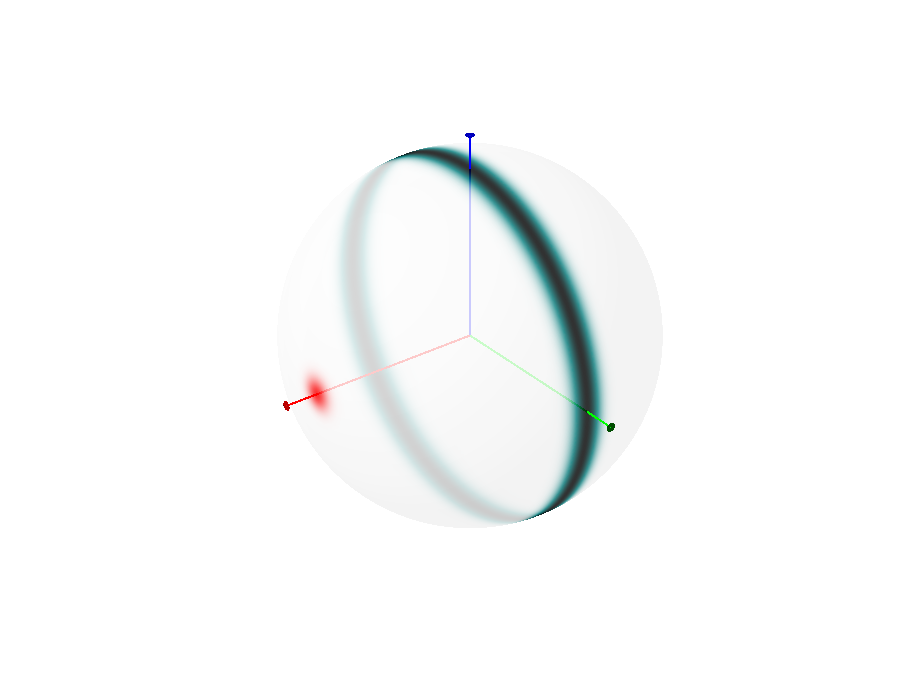
\includegraphics[width=0.20\textwidth, trim=115 60 95 20, clip]{est_LI_F1}
				} \hspace{-0.2cm}
				\subfigure{
					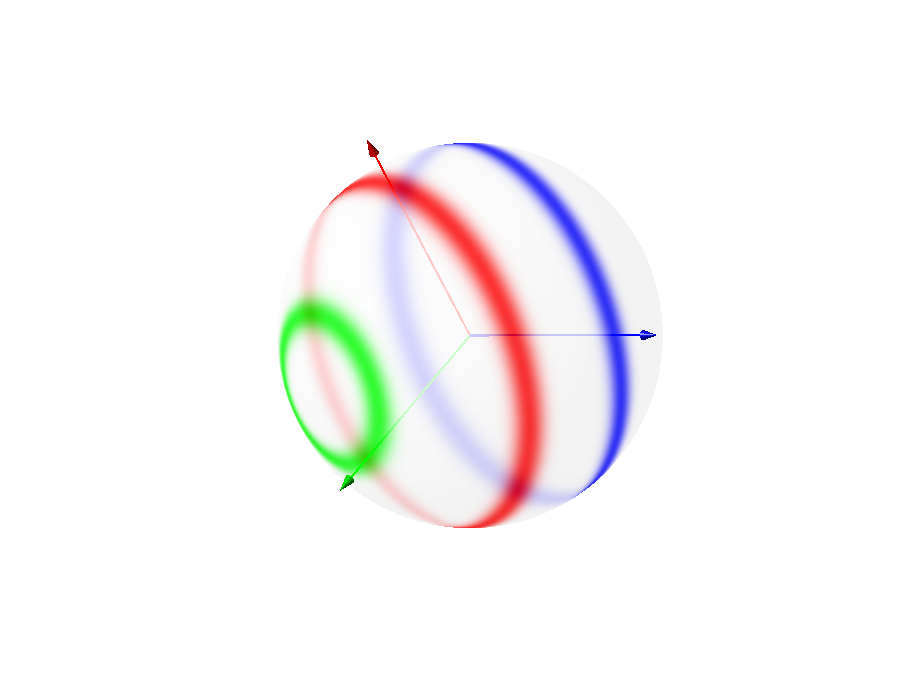
\includegraphics[width=0.20\textwidth, trim=115 60 95 20, clip]{est_LI_F5}
				} \hspace{-0.2cm}
				\subfigure{
					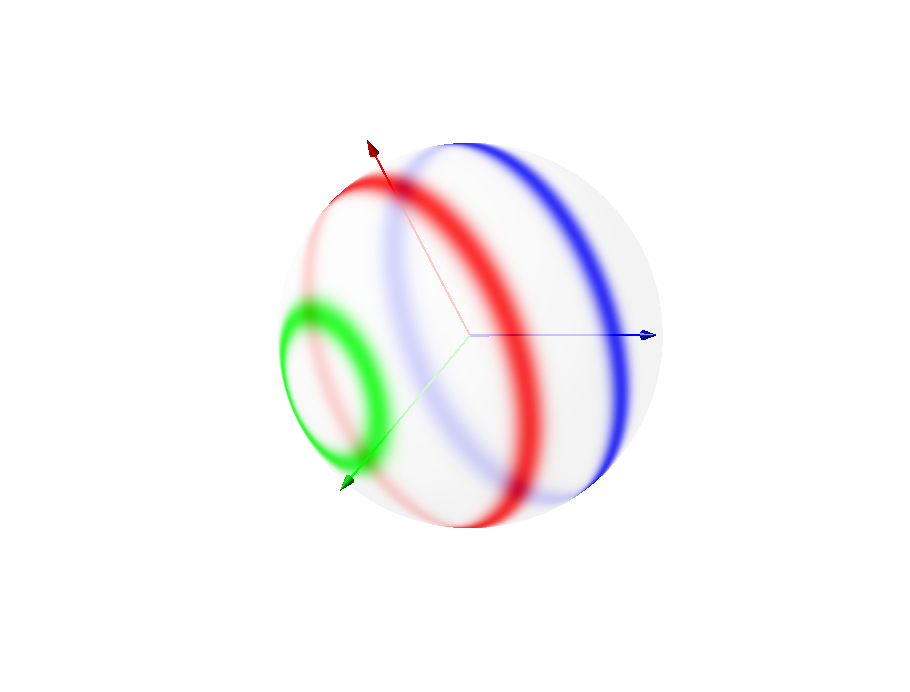
\includegraphics[width=0.20\textwidth, trim=115 60 95 20, clip]{est_LI_FN_mea}
				} \hspace{-0.2cm}
				\subfigure{
					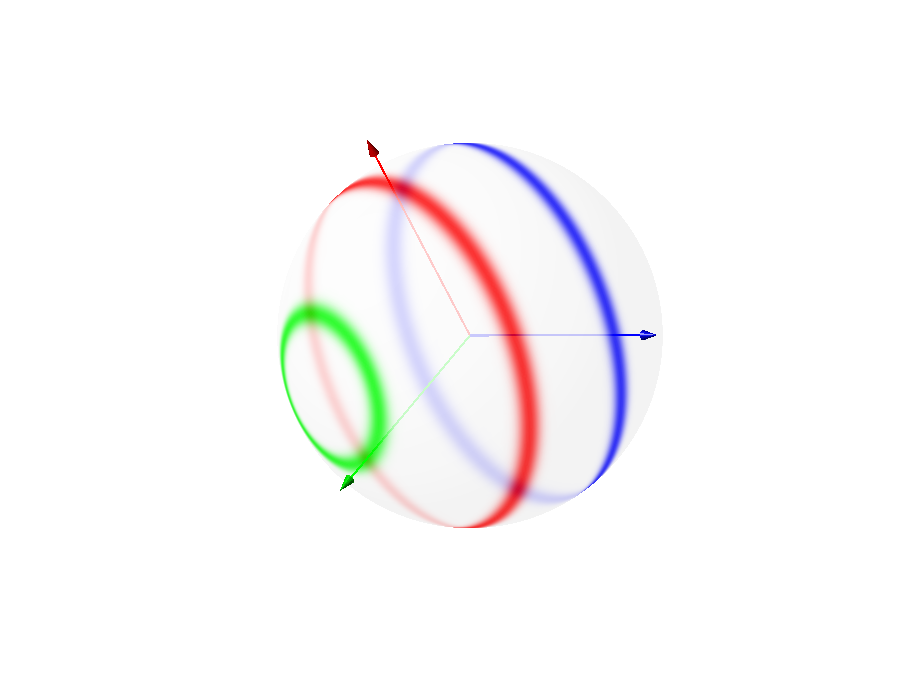
\includegraphics[width=0.20\textwidth, trim=115 60 95 20, clip]{est_LI_FN_post}
				}
			}
			\begin{tikzpicture}[overlay]
				\node at (-5.0,0.2) {\tiny Prior dist. at $t=0$};
				\node at (-2.65,0.2) {\tiny Posterior dist. at $t=0$};
				\node at (-0.3,0.2) {\tiny Propagated dist. at $t=1$};
				\node at (2.05,0.2) {\parbox{0.2\textwidth}{\tiny Propagated dist. overlapped \\ with measured dist. at $t=1$}};
				\node at (4.4,0.2) {\tiny Posterior dist. at $t=1$};
				
				\draw[arrows={-Triangle[angle=30:2pt]}] (-3.85,0.8) -- ++(90:0.3);
				\draw[arrows={-Triangle[angle=30:2pt]}] (-3.85,0.8) -- ++(-30:0.3);
				\draw[arrows={-Triangle[angle=30:2pt]}] (-3.85,0.8) -- ++(210:0.3);
				\node at (-4.15,0.5) {\tiny $\mathbf{e}_1$};
				\node at (-3.45,0.5) {\tiny $\mathbf{e}_2$};
				\node at (-3.82,1.23) {\tiny $\mathbf{e}_3$};
			\end{tikzpicture}
		\end{figure}
	\end{itemize}
\end{frame}

\subsection{Attitude Estimation Based on MFG}

\begin{frame}
	\frametitle{Problem Formulation}
\end{frame}

\section{6D Pose Estimation With MFG}



\end{document}


